\documentclass[11pt,a4paper]{article}

\usepackage[utf8]{inputenc}
\usepackage[T1]{fontenc}
\usepackage{lmodern}
\usepackage{microtype}
\usepackage[margin=2.5cm]{geometry}
\usepackage{amsmath,amssymb,amsthm}
\usepackage{mathtools}
\usepackage{bm}
\usepackage{graphicx}
\usepackage{booktabs}
\usepackage{array}
\usepackage{tabularx}
\usepackage{longtable}
\usepackage{multirow}
\usepackage{enumitem}
\usepackage{xcolor}
\usepackage{tikz}
\usetikzlibrary{arrows.meta,positioning,calc,shapes.geometric,fit}
\usepackage[numbers,sort&compress]{natbib}
\usepackage[hidelinks]{hyperref}
\usepackage[capitalise,noabbrev]{cleveref}
\usepackage{caption}
\captionsetup{font=small,labelfont=bf,width=0.95\linewidth}
\setlength{\emergencystretch}{3em}

\hypersetup{
  pdftitle={Circuit knowledge graphs: reactions as element laws, typed verdicts in place of inference, and a pre-registered audit of human cytosolic biochemistry},
  pdfauthor={Kundai Farai Sachikonye}
}

\newtheorem{definition}{Definition}
\newtheorem{proposition}{Proposition}
\newtheorem{lemma}{Lemma}
\theoremstyle{remark}
\newtheorem{remark}{Remark}

\newcommand{\kJ}{\ensuremath{\,\mathrm{kJ\,mol^{-1}}}}
\newcommand{\DG}{\ensuremath{\Delta_r G^\circ}}
\newcommand{\DGp}{\ensuremath{\Delta_r G'^\circ}}
\newcommand{\DGm}{\ensuremath{\Delta_r G'_{\mathrm{m}}}}
\newcommand{\vd}[1]{\textsf{#1}}
\newcommand{\conv}[1]{\texttt{#1}}
\newcommand{\im}{\operatorname{im}}
\newcommand{\rank}{\operatorname{rank}}

\begin{document}

\title{\textbf{Circuit Knowledge Graphs}\\[6pt]
{\Large Reactions as Element Laws, Typed Verdicts in Place of Inference,\\ and a Pre-registered Audit of Human Cytosolic Biochemistry}}

\author{
Kundai Farai Sachikonye\\
Technical University of Munich, School of Life Sciences\\
\texttt{kundai.sachikonye@wzw.tum.de}
}

\date{\today}

\maketitle

\begin{abstract}
\noindent
Knowledge graphs of biochemistry store curated assertions and answer questions by inference.
Inference under an open world cannot tell a fact that is false from a fact that was never measured.
We describe a \emph{circuit knowledge graph}, in which reactions are junctions carrying element laws and species are nodes whose values are the solutions of those laws.
The cytosolic medium is the electrical ground.
Every computation returns a typed verdict instead of an inferred triple: \vd{answered}, \vd{certified-empty}, \vd{absent}, \vd{underdetermined}, \vd{undecidable}, \vd{refused} or \vd{subfloor}.
A verdict other than \vd{answered} carries no payload and names its blocker.
Each value carries a provenance basis that composes without laundering, and each empty answer carries a letter saying why it is empty.
We built the graph over the 2{,}914 human reactions in Reactome whose every participant and modifier is cytosolic.
We joined them to measured reaction thermodynamics, kinetic constants, protein abundances, AlphaFold structures and thirteen further curated resources.
The analyses were organised around 23 claims written down and committed before the code that tested them was run.
Measured thermodynamics determine only 75 of the 2{,}914 reactions; Hess's law adds 30 and a carrier/slot decomposition of protein phosphorylation adds 96.
Under the cytosolic window of pH, ionic strength and free magnesium, the direction of 156 of 199 undecided reactions is blocked by concentrations alone.
The 17 disagreements with curated directions are reactions that run uphill at 1\,mM.
Enzymes leave the dilute regime at a median of 2.4\,\textmu M, so enzyme--substrate states cannot be folded into metabolite capacitances.
AlphaFold contact graphs agree with crystal structures (median Jaccard index 0.90, against 0.14 for a shifted control).
A coupled-oscillator account of folding fails every test it was given.
Of the 23 pre-registered claims, 14 held, 8 failed and 1 could not be tested for want of data.
The failures are as informative as the successes, because each verdict states what would decide it.
\end{abstract}

\noindent\textbf{Keywords:} knowledge graphs; reaction networks; network thermodynamics; Legendre transform; Hess's law; provenance; AlphaFold; pre-registration; three-valued logic.

\tableofcontents
\clearpage

%==============================================================================
\section{Introduction}
\label{sec:intro}

Curated pathway resources describe human biochemistry as a graph of typed assertions.
Reactome states which entities take part in a reaction, in which compartment and with which catalyst \citep{gillespie2022reactome}.
Rhea states balanced reaction equations over a chemical ontology \citep{bansal2022rhea}.
Genome-scale models such as Human-GEM state stoichiometric matrices with bounds on fluxes \citep{robinson2020humangem}.
A knowledge graph built on such resources answers a question by inference over its triples \citep{hogan2021knowledge}.

Inference has two weaknesses for a physical system.
The first is semantic.
Under the open-world assumption, the absence of a triple means nothing; under the closed-world assumption, it means that the fact is false.
Neither reading matches what a biochemist needs to know: whether a value was measured and found to be empty, never measured, outside the scope of the source, or measured but too noisy to decide.
The second weakness is physical.
A reaction network is not an arbitrary relational structure.
Its stoichiometric matrix fixes conservation laws, steady flux modes and thermodynamic cycles independently of any rate constant \citep{feinberg2019foundations,schuster1994efm}.
Its reactions are driven by affinities, which are differences of chemical potential, exactly as currents in an electrical network are driven by differences of voltage \citep{oster1971network,schnakenberg1976network}.
An inference engine that treats a reaction as a labelled edge discards this structure.

This paper describes a kernel that keeps it.
In a \emph{circuit knowledge graph}, each reaction is a junction whose edges carry element laws: mass-action flux in flux--force form, and Kirchhoff's current law at every species.
A species' value, its chemical potential, is never stored.
It is whatever solves the node's law from the node's contacts, and when the data needed to solve it are missing, the answer is a verdict that names what is missing.
The cytosol is the electrical ground: ambient cofactors are folded into a single medium vertex, and every item touches it.
This reading follows the network thermodynamics of \citet{oster1971network}, and it keeps the energetic constraints that thermodynamics-based flux analysis imposes \citep{beard2002energy,henry2007tfba} as structural facts rather than optimisation constraints.

The central design decision is that nothing is inferred.
Every function returns a typed verdict (\cref{sec:verdicts}).
A verdict other than \vd{answered} may not carry a payload, and must name its blocker; this is enforced by the type, not by convention.
The labels distinguish a well-posed question with an empty answer (\vd{certified-empty}) from a question whose required datum is missing (\vd{absent}).
They also separate several admissible readings with no rule to select one (\vd{underdetermined}) from data that cannot resolve the answer within tolerance (\vd{undecidable}).
A question the graph cannot state is \vd{refused}, and a composite power below its declared target is \vd{subfloor}.
On top of the label, every value carries a provenance basis (stated, supplied, derived or estimated) that composes as a maximum and therefore cannot be laundered.
Every empty answer carries a letter that says why it is empty, and every fact carries a ground verdict computed from its provenance chain.

We built the kernel over the 2{,}914 Reactome reactions whose every reactant, product and modifier lies in the cytosol.
We then extended it, stage by stage, with public measurements.
The measurements are equilibrium constants from the Thermodynamics of Enzyme-Catalyzed Reactions Database (TECRDB) \citep{goldberg2004tecrdb}, transformed to cytosolic conditions with eQuilibrator's Legendre transform \citep{alberty2003thermodynamics,beber2022equilibrator}.
They include kinetic constants from the System for the Analysis of Biochemical Pathways -- Reaction Kinetics (SABIO-RK) \citep{wittig2012sabio} and protein abundances from PaxDb \citep{wang2015paxdb}.
They include protein structures from the AlphaFold Protein Structure Database \citep{jumper2021alphafold,varadi2022afdb} and the Protein Data Bank \citep{berman2000pdb}.
Finally, they include cross-references, localisation, residue annotations and disorder from Rhea, MetaNetX, Human-GEM, the Human Protein Atlas, COMPARTMENTS, UniProt, the Mechanism and Catalytic Site Atlas (M-CSA) and DisProt \citep{bansal2022rhea,moretti2021metanetx,robinson2020humangem,thul2017hpa,binder2014compartments,uniprot2023,ribeiro2018mcsa,quaglia2022disprot}.

Each extension was organised around claims that were written down, with the outcome that would count against them, and committed to version control before the code that tested them existed \citep{nosek2018preregistration}.
Several of those claims failed.
We report every outcome, and we treat a failed claim as a result.

\paragraph{Contributions.}
\begin{enumerate}[leftmargin=*,itemsep=2pt]
  \item A formal model of a biochemical knowledge graph in which edges are element laws, node values are solutions, the medium is ground, and answers are typed verdicts with non-launderable provenance (\cref{sec:model}).
  \item Structural results that hold without any rate constant: rank, conservation laws and blocked junctions; a three-valued cycle test with explicit tolerances; the determinacy condition for Hess's law; and a guard that refuses cycle tests which cannot fail (\cref{sec:model,sec:construction}).
  \item Separation costs on counted weights, with a proof that attaching new structure never lowers them, and a control showing that real-valued weights do (\cref{sec:cuts,sec:res-proteins}).
  \item A complete construction from public data, with every supplied convention named on the values it produces (\cref{sec:construction,app:conventions}).
  \item A pre-registered audit of 23 claims across seven stages, with outcomes, controls and the reasons for each failure (\cref{sec:protocol,sec:results}).
\end{enumerate}

\paragraph{Principal findings.}
Measured thermodynamics determine 75 of the 2{,}914 reactions directly; Hess's law and a carrier/slot decomposition raise this to 201 (\cref{sec:res-thermo}).
For 156 of the 199 reactions whose direction is undecided, the cytosolic medium fixes the sign of the affinity at 1\,mM, so only concentrations block the answer (\cref{sec:res-medium}).
Where the kernel disagrees with curated directions, the reactions are those that run uphill at 1\,mM and are pulled forward by product removal (\cref{sec:res-db}).
Enzymes are not dilute: their sites saturate at micromolar substrate (\cref{sec:res-kinetics}).
AlphaFold contact graphs reproduce crystal-structure contacts, and catalytic residues are contact hubs within them (\cref{sec:res-db}).
A coupled-oscillator account of folding adds nothing to the contact graph it runs on (\cref{sec:res-folding}).

%==============================================================================
\section{Background and related work}
\label{sec:related}

\paragraph{Pathway knowledge bases and genome-scale models.}
Reactome curates reactions as events over physical entities in compartments, with catalysts and regulators as modifiers \citep{gillespie2022reactome}.
Rhea curates balanced equations over the Chemical Entities of Biological Interest (ChEBI) ontology \citep{bansal2022rhea,hastings2016chebi}.
MetaNetX reconciles the namespaces of metabolic models \citep{moretti2021metanetx}.
Human-GEM is a consensus genome-scale model of human metabolism \citep{robinson2020humangem}.
Flux balance analysis optimises an objective over the null space of such a matrix under flux bounds \citep{orth2010fba}.
The circuit knowledge graph shares the stoichiometric matrix with these models, but it does not optimise; it reports what the matrix and the measurements determine, and names what they leave open.

\paragraph{Thermodynamics of reaction networks.}
Network thermodynamics represents a reaction network as an electrical circuit whose currents are fluxes and whose potentials are chemical potentials \citep{oster1971network}.
Schnakenberg's cycle decomposition gives the entropy production of a network as a sum over cycle affinities \citep{schnakenberg1976network}.
Later work treats open networks with emergent cycles and broken conservation laws \citep{polettini2014irreversible,rao2016nonequilibrium}.
Energy-balance analysis \citep{beard2002energy} and thermodynamics-based flux analysis \citep{henry2007tfba} require that no flux mode run around a cycle with zero net affinity.
Network-embedded thermodynamic analysis checks metabolome data for consistency with these constraints \citep{kummel2006net}.
Our kernel takes the element-law reading literally: each junction's law and each node's law are the edges and vertices of the graph.

\paragraph{Gibbs energies of reaction.}
Measured apparent equilibrium constants are collected in TECRDB \citep{goldberg2004tecrdb}.
Transforming them between conditions requires Alberty's Legendre transform over the microspecies of each reactant \citep{alberty1998calculation,alberty2003thermodynamics}.
Group-contribution and component-contribution methods estimate formation energies for compounds that were never measured \citep{jankowski2008group,noor2013component}.
eQuilibrator implements both \citep{flamholz2012equilibrator,beber2022equilibrator}.
We use eQuilibrator's microspecies data and transform, but deliberately not its estimates: a value that a model predicted carries the basis \vd{estimated} and is never reported as measured (\cref{sec:basis}).
We also show that cycle tests built only from species-level energies are non-falsifiable, which is why the kernel's cycle test uses reaction-level measurements only (\cref{prop:falsifiable}).

\paragraph{Metabolite concentrations, kinetics and abundance.}
Absolute concentrations of central metabolites have been measured in bacteria, yeast and mammalian cells \citep{bennett2009absolute,park2016concentrations}.
Kinetic constants are collected in SABIO-RK and the BRaunschweig ENzyme DAtabase (BRENDA) \citep{wittig2012sabio,chang2021brenda}; their in vitro values relate only loosely to in vivo rates \citep{davidi2016global}, and their distribution is broad \citep{bareven2011moderately}.
Protein abundances are integrated across studies in PaxDb \citep{wang2015paxdb}.
Total protein concentration constrains the conversion from parts per million to molar \citep{milo2013protein}.
Macromolecular crowding reduces the volume available to solutes \citep{minton2001crowding,zhou2008crowding}.

\paragraph{Protein structure.}
AlphaFold predicts structures with per-residue confidence \citep{jumper2021alphafold}, and its database covers the human proteome \citep{tunyasuvunakool2021human,varadi2022afdb}.
Low-confidence regions coincide with intrinsic disorder \citep{ruff2021alphafold}, which in turn is enriched at phosphorylation sites \citep{iakoucheva2004disorder}.
Solvent accessibility follows the Shrake--Rupley construction \citep{shrake1973environment}; secondary structure follows the hydrogen-bond assignment of \citet{kabsch1983dssp}.
Sequence-only contact prediction has a long history, of which coevolutionary coupling is the best-established form \citep{morcos2011dca}.

\paragraph{Missing values, provenance and verdicts.}
Strong Kleene logic gives a third truth value for propositions whose value is not determined \citep{kleene1952introduction}.
The verdict labels refine that third value by its cause.
Provenance standards such as the Provenance Ontology (PROV-O) of the World Wide Web Consortium record which activity generated which entity from which inputs \citep{lebo2013provo}.
We compute a ground verdict from such a chain, using Peirce's distinction between symbol, index and icon \citep{peirce1932collected} to say whether a fact rests on a measurement of its object, on a model of it, or on neither.
The verdicts make data reuse more honest in the sense of the principles that data be findable, accessible, interoperable and reusable \citep{wilkinson2016fair}: a reused value carries the conditions under which it is valid.

%==============================================================================
\section{The circuit knowledge graph}
\label{sec:model}

\subsection{Vertices, edges and element laws}
\label{sec:graph}

\begin{definition}[Circuit knowledge graph]
\label{def:ckg}
A circuit knowledge graph is an undirected weighted graph $G=(V,E,w)$ with $V = S \cup R \cup \{M\}$, where $S$ is the set of species vertices, $R$ the set of junction (reaction) vertices and $M$ the medium vertex.
Its edges are of four kinds:
\begin{enumerate}[label=(\roman*),itemsep=1pt]
  \item a \emph{stoichiometric edge} $\{s,r\}$ with signed coefficient $\nu_{sr}\neq0$, weight $|\nu_{sr}|$;
  \item a \emph{modifier edge} $\{s,r\}$ for a catalyst, stimulator or inhibitor, with $\nu_{sr}=0$ and unit weight;
  \item a \emph{junction medium edge} $\{r,M\}$, of weight $1+\sum_{a\in A_r}|\nu_{ar}|$, where $A_r$ is the set of ambient species of $r$ folded into $M$;
  \item a \emph{species medium edge} $\{s,M\}$ of unit weight, for every $s\in S$.
\end{enumerate}
The state of a species vertex is its chemical potential $\mu_s=\mu_s^\circ+RT\ln c_s$.
The state of a junction is its affinity $A_r=-\sum_s \nu_{sr}\mu_s$ and its flux $J_r$.
\end{definition}

The edges carry the differential equations of the network.
The junction element law is mass action written in flux--force form:
\begin{equation}
  J_r \;=\; k_r \prod_{s:\,\nu_{sr}<0} c_s^{|\nu_{sr}|}\,\Bigl(1-e^{-A_r/RT}\Bigr),
  \label{eq:junction}
\end{equation}
whose tangent at equilibrium is the linear law $J_r = G_r A_r$ with conductance $G_r$.
The node law is Kirchhoff's current law, which is mass balance:
\begin{equation}
  \frac{c_s}{RT}\,\frac{d\mu_s}{dt} \;=\; \sum_{r} \nu_{sr} J_r \;\bigl(+\,G^{\mathrm{ex}}_s(\mu^{\mathrm{res}}_s-\mu_s)\ \text{if $s$ exchanges with a reservoir}\bigr).
  \label{eq:node}
\end{equation}
Here $c_s/RT$ is the node's capacitance.
Modifier edges carry no current; they enter the prefactor $k_r$ of \cref{eq:junction}.
\Cref{fig:schema} shows the elements.

\begin{figure}[t]
\centering
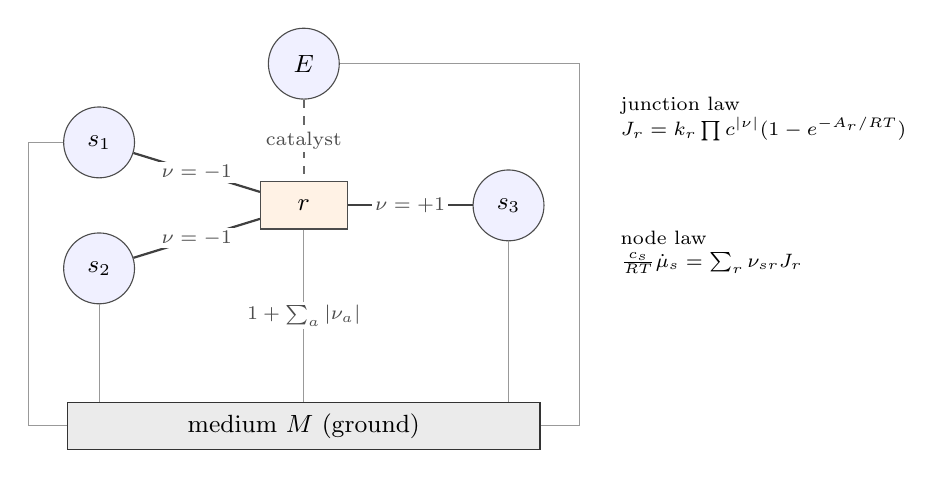
\begin{tikzpicture}[
  sp/.style={circle,draw=black!70,fill=blue!6,minimum size=9mm,inner sep=0pt,font=\small},
  jn/.style={rectangle,draw=black!70,fill=orange!10,minimum width=11mm,minimum height=6mm,font=\small},
  md/.style={rectangle,draw=black!80,fill=black!8,minimum width=60mm,minimum height=6mm,font=\small},
  st/.style={-,thick,black!75},
  mo/.style={-,thick,dashed,black!60},
  me/.style={-,thin,black!40},
  lab/.style={font=\scriptsize,black!70,fill=white,inner sep=1pt}
]
\node[sp] (s1) at (0,1.6) {$s_1$};
\node[sp] (s2) at (0,0) {$s_2$};
\node[jn] (r) at (2.6,0.8) {$r$};
\node[sp] (s3) at (5.2,0.8) {$s_3$};
\node[sp] (e) at (2.6,2.6) {$E$};
\node[md] (M) at (2.6,-2.0) {medium $M$ (ground)};
\draw[st] (s1) -- node[lab]{$\nu=-1$} (r);
\draw[st] (s2) -- node[lab]{$\nu=-1$} (r);
\draw[st] (r) -- node[lab]{$\nu=+1$} (s3);
\draw[mo] (e) -- node[lab]{catalyst} (r);
\draw[me] (s1.west) -- (-0.9,1.6) |- (M.west);
\draw[me] (s2) -- (s2 |- M.north);
\draw[me] (r) -- node[lab]{$1+\sum_{a}|\nu_{a}|$} (r |- M.north);
\draw[me] (s3) -- (s3 |- M.north);
\draw[me] (e.east) -- (6.1,2.6) |- (M.east);
\node[font=\scriptsize,align=left,anchor=west] at (6.5,1.9) {junction law\\$J_r = k_r\prod c^{|\nu|}(1-e^{-A_r/RT})$};
\node[font=\scriptsize,align=left,anchor=west] at (6.5,0.2) {node law\\$\frac{c_s}{RT}\dot\mu_s=\sum_r\nu_{sr}J_r$};
\end{tikzpicture}
\caption{Elements of a circuit knowledge graph.
Species (circles) carry potentials, junctions (rectangle) carry affinity and flux, and the medium $M$ is ground.
Solid edges are stoichiometric contacts with signed coefficients, the dashed edge is a modifier contact, and thin edges connect every item to the medium.
Ambient cofactors (water, the proton, orthophosphate and eleven others; \cref{sec:medium-ground}) are folded into $M$, which raises the weight of the junction's medium edge.}
\label{fig:schema}
\end{figure}

\subsection{The medium as ground}
\label{sec:medium-ground}

Fourteen small molecules are declared ambient.
They are water, the proton, orthophosphate, pyrophosphate, carbon dioxide, dioxygen and coenzyme~A.
They also include adenosine triphosphate (ATP), adenosine diphosphate (ADP) and adenosine monophosphate (AMP).
The last four are nicotinamide adenine dinucleotide (NAD) as NAD$^+$ and reduced NAD (NADH), and NAD phosphate (NADP) as NADP$^+$ and reduced NADP (NADPH).
Their potentials are taken as fixed by the cytosol, so they are not items; they are folded into $M$ (convention \conv{ambient-reservoir}).
The list is a declaration, not a finding.
Changing the list changes every downstream number, which is why the list is part of the stage digest (\cref{sec:digests}).
Every item has an edge to $M$ (convention \conv{medium-floor}), so every item is connected to ground and every separation cost of \cref{sec:cuts} is finite and positive.

\subsection{Structure without parameters}
\label{sec:structure}

Let $N$ be the stoichiometric matrix restricted to the internal species, with one column per junction.
Its rank, its left null space (conservation laws) and its right null space (steady flux modes) are properties of the system of node laws that do not depend on any rate constant.

\begin{proposition}[Blocked junctions]
\label{prop:blocked}
Hold the medium and every species not in $N$ at fixed potential.
Junction $r$ carries zero flux in every steady state of the node laws if and only if $e_r^{\top} v = 0$ for every $v\in\ker N$.
\end{proposition}
\begin{proof}
At steady state $\dot\mu_s=0$ for every internal species, so by \cref{eq:node} $NJ=0$, i.e.\ $J\in\ker N$.
If every $v\in\ker N$ has $v_r=0$, then $J_r=0$.
Conversely, if some $v\in\ker N$ has $v_r\neq0$, then $J=v$ satisfies the steady-state balance with $J_r\neq0$.
\end{proof}

In practice, an orthonormal basis $V_0$ of $\ker N$ is taken from a singular value decomposition, and $r$ is blocked when row $r$ of $V_0$ has norm below $10^{-8}$.
The numerical rank is cut at a relative singular value of $10^{-9}$.
The cut is rejected unless it falls inside a spectral gap: if the largest dropped singular value exceeds $10^{-12}$ of the largest and the smallest kept one is below $10^{-6}$ of it, the computation stops with an error.
A size-scaled cut (the common default $\epsilon\max(m,n)\sigma_1$) fell above the smallest genuine singular value of the enzyme-expanded matrix and invented null vectors; the gap rule exists because of that failure, and a regression test pins it.

\subsection{Verdicts}
\label{sec:verdicts}

\begin{definition}[Verdict]
\label{def:verdict}
A verdict is a tuple $(\ell, p, b, \rho, \delta, g)$ of a label $\ell$, a payload $p$, a blocker $b$, a remedy $\rho$, a detail record $\delta$ and an optional gate letter $g$.
The label takes one of seven values.
The label \vd{answered} means a payload is present, and \vd{certified-empty} that the question is well posed and its answer is empty.
The label \vd{absent} means a required datum is absent.
The label \vd{underdetermined} means several readings are admissible and no rule selects one.
The label \vd{undecidable} means the data cannot resolve the answer within tolerance.
The label \vd{refused} means the question is outside what the graph can state, and \vd{subfloor} that a composite power is below its declared target.
\end{definition}

Two invariants are enforced at construction time, so a verdict that violates them cannot exist:
\begin{enumerate}[label=(V\arabic*),itemsep=1pt]
  \item if $\ell\neq\vd{answered}$ then $p$ is empty;
  \item if $\ell\notin\{\vd{answered},\vd{certified-empty}\}$ then $b$ is non-empty.
\end{enumerate}
(V1) prevents a missing value from travelling downstream disguised as a number.
(V2) makes every non-answer actionable, because its blocker says what is missing and its remedy, when present, says what would supply it.
A gate letter (\cref{sec:gates}) may be attached only to \vd{certified-empty} or \vd{absent} verdicts.

The labels refine the third value of strong Kleene logic by cause \citep{kleene1952introduction}.
\vd{absent} and \vd{undecidable} both leave the answer open, but they ask for different remedies.
The first needs a new measurement; the second needs a more precise one.
A \vd{certified-empty} verdict closes the question: a completion search that finds no route has answered it.
A \vd{refused} verdict is not a failure of data at all: TECRDB states only small-molecule reactions, so asking it for the $\DG$ of a reaction with a protein participant is outside its scope.

\subsection{Provenance}
\label{sec:provenance}

\subsubsection{Basis}
\label{sec:basis}

Every value carries a basis tag: \emph{stated} (the source record asserts it), \emph{supplied} (a named convention produced it) or \emph{derived} (the kernel computed it from other values).
A fourth tag, \emph{estimated}, marks a value a model predicted, for instance by component contribution \citep{noor2013component} or as a learned turnover number \citep{li2022dlkcat}.
A fifth tag, \emph{absent}, marks a value that neither source nor convention determines.
A supplied value must name its convention; an absent value carries none.

\begin{proposition}[Basis is never laundered]
\label{prop:basis}
Order the bases \emph{stated} $<$ \emph{supplied} $<$ \emph{derived} $<$ \emph{estimated}, and let the composition of tags be their maximum, with \emph{absent} absorbing.
Then the composition is associative, commutative and idempotent, and no value computed from an estimated or derived input can carry a lower basis.
\end{proposition}
\begin{proof}
The maximum over a total order is a join on a chain, hence a semilattice operation; adjoining an absorbing element preserves associativity, commutativity and idempotence.
Monotonicity of the maximum gives the second statement.
\end{proof}

Of the 201 reactions with a chemical-reference $\DG$ (\cref{sec:res-thermo}), 75 direction verdicts are \emph{supplied} (a measured value judged under the supplied medium window) and 126 are \emph{derived}; none can be reported as stated.

\subsubsection{Gate letters for empty answers}
\label{sec:gates}

An empty or absent answer can be empty for different reasons, and the reasons matter for what to do next.
Each such verdict carries one of five letters.
The letter $+$ means witnessed absent: the source covers the case and records nothing.
The letter $-$ means not recorded: the source does not cover it, and \textsf{a} means both.
\textsf{open} means a name the source never uses, so the question cannot be put to it, and \textsf{?} means undecided.
The letter is assigned from the blocker by a fixed rule table; a \vd{certified-empty} answer defaults to $+$ because it completed and found nothing.
For example, ``no TECRDB measurement of this reaction'' is $-$, while ``participant without an identifier of the Kyoto Encyclopedia of Genes and Genomes (KEGG)'' is \textsf{open}.
The second can be closed by a cross-reference, the first only by a measurement (\cref{sec:res-db}).

\subsubsection{Ground verdicts}
\label{sec:ground}

Each fact family is generated by a typed activity that used other records, forming a provenance chain in the sense of PROV-O \citep{lebo2013provo}.
Walking the chain backwards, three bits are collected: $g$ (a generation is recorded), $c$ (a contact activity, i.e.\ a measurement of the object, is reachable) and $d$ (a derivation is reachable).
The ground verdict is
\begin{center}
\begin{tabular}{@{}cccl@{}}
\toprule
$g$ & $c$ & $d$ & ground verdict \\
\midrule
0 & 0 & 0 & symbol (nothing generated it) \\
1 & 0 & 0 & collapsed (curation with no contact) \\
1 & 1 & 0 & index (a measurement of the object) \\
1 & 0 & 1 & icon (a model of the object) \\
1 & 1 & 1 & composite (measurement and derivation) \\
\bottomrule
\end{tabular}
\end{center}
with an override: if any model prediction (component contribution, machine-learned prediction, group contribution) is reachable, the verdict is \emph{estimated}.
The terms follow Peirce's division of signs by their relation to their object \citep{peirce1932collected}: an index is physically connected to its object, an icon resembles it, a symbol relates to it by convention only.
Over the kernel's fact families, TECRDB rows, SABIO-RK parameters, PaxDb abundances and Protein Data Bank coordinates are indices.
Every pooled or derived $\DG$, every direction verdict, every retention factor and every distance measured on a crystal structure is composite.
AlphaFold models, and the contact graphs and enzyme cycles built on them, are icons.
Reactome stoichiometry, UniProt Enzyme Commission (EC) numbers and eQuilibrator microspecies tables are collapsed.
The chemical potential $\mu$, which is never stored, is a symbol.

\subsubsection{Stage digests}
\label{sec:digests}

A derived value is valid only for the content and conventions it was computed on.
Each stage records a digest: the SHA-256 of each input file, the SHA-256 of the canonical serialisation of its conventions, and the SHA-256 of both together.
A stage is current if recomputing the digest reproduces it.
Changing the pH window makes the medium stage stale; the check is discriminating because its control (an unchanged window) stays current.

\subsubsection{Check markers}
\label{sec:checks}

A check is reported as \emph{pass}, \emph{fail}, \emph{non-discriminating} or \emph{uncontrolled}.
It is non-discriminating when its control passes as well: a test that cannot fail tells nothing.
Every test in the kernel's suite (\cref{app:tests}) has a control that must change the outcome.

\subsection{Counted weights and separation costs}
\label{sec:cuts}

All edge weights used for cuts are counts: stoichiometric coefficients, heavy-atom contacts, exposed atoms.
Real-valued quantities such as Gibbs energies or conductances stay in the element laws and never become cut weights.

\begin{definition}[Local cut key]
\label{def:cutkey}
Let $H=G-M$ be the item graph and $B_r(v)$ the ball of radius $r$ about item $v$ in $H$.
Build a flow network on $B_r(v)$ with the edge weights of $G$ as capacities, and join every edge from $B_r(v)$ to a vertex outside it (including $M$) to a single sink $T$.
The \emph{local separation cost} $\sigma_r(v)$ is the maximum flow from $v$ to $T$, equal to the minimum cut \citep{ford1956maximal}.
Write $\delta_r(v)$ for the size of the source side of the minimal minimum cut, $\beta_r(v)$ for the smallest edge weight inside the ball or on its medium edges, and $\pi_r(v)=1-\beta_r(v)/\sigma_r(v)$ for the derived power.
The cut key of $v$ is $(\sigma_r,\delta_r)$.
\end{definition}

Maximum flows are computed by preflow--push \citep{goldberg1988preflow}; the source side of the minimal cut is the set reachable from $v$ in the residual network.
The \emph{global separation cost} $\sigma(v)$ is the maximum flow from $v$ to $M$ in the connected component of $v$.

\begin{proposition}[Expansion never lowers separation cost]
\label{prop:monotone}
Let $G'$ be obtained from $G$ by adding vertices and edges with non-negative weights, without changing any existing weight.
Then $\sigma_{G'}(v)\ge\sigma_G(v)$ for every vertex $v$ of $G$.
\end{proposition}
\begin{proof}
Let $(X',\bar X')$ be a minimum $v$--$M$ cut in $G'$ and $X=X'\cap V(G)$.
Every edge of $G$ crossing $(X,V(G)\setminus X)$ also crosses $(X',\bar X')$ in $G'$ with the same weight, so the cut value of $X$ in $G$ is at most that of $X'$ in $G'$.
Hence $\sigma_G(v)\le\sigma_{G'}(v)$.
\end{proof}

The proposition is why proteins are attached to the graph by expansion (\cref{sec:attach}): new residue vertices and edges only.
It does not cover the tempting alternative of replacing an existing counted weight by a real-valued one, and \cref{sec:res-proteins} shows that this alternative does lower separation costs.

\paragraph{Colour refinement.}
Classes of structurally equivalent items are computed by colour refinement \citep{weisfeiler1968reduction}.
The initial colour of an item is (kind, $\sigma_1$, $\delta_1$); each round replaces the colour by the pair (colour, sorted multiset of (edge role, edge weight, neighbour colour)).
Labels are canonical: colours are ranks of sorted signatures.

\begin{proposition}[Refinement is invariant and monotone]
\label{prop:refine}
The final partition is invariant under any relabelling of the items, and the partition after each round refines the one before.
\end{proposition}
\begin{proof}
Every quantity entering a colour is a function of the weighted, role-labelled graph alone, and canonical ranking removes any dependence on item names; hence an isomorphism maps classes to classes.
The new colour contains the old colour as a component, so two items with different old colours have different new colours.
\end{proof}

Refinement stops when the number of classes no longer grows.
Items left in a shared class cannot be separated by any number of further rounds, just as two analytes of equal retention cannot be separated by any column length \citep{giddings1991unified}.
The information still needed to locate an item within its class is $\log_2 s$ bits for a class of size $s$.
With $n_c$ distinct values of the initial key, at least $\log K/\log n_c$ independent keys are needed to give $K$ items distinct positions.

\subsection{Ladders}
\label{sec:ladders}

A series chain reservoir $\to r_1\to s_1\to\cdots\to r_n\to s_n\to M$ in the linear tangent $J=GA$ has resistances $R_k=1/G_k$ and a medium exchange resistance $R_M$.
Define the power of rung $k$ as the fraction of the remaining drop it closes:
\begin{equation}
  \pi_k = \frac{R_k}{R_k+R_{k+1}+\cdots+R_n+R_M}.
\end{equation}

\begin{proposition}[Ladder powers telescope]
\label{prop:ladder}
With $R_{\mathrm{tot}}=\sum_k R_k + R_M$, the composite power is $1-\prod_k(1-\pi_k) = 1-R_M/R_{\mathrm{tot}}$, and the share $R_k/R_{\mathrm{tot}}$ of rung $k$ equals its flux control coefficient $\partial\ln J/\partial\ln G_k$.
\end{proposition}
\begin{proof}
$1-\pi_k=(R_{k+1}+\cdots+R_M)/(R_k+\cdots+R_M)$, so the product telescopes to $R_M/R_{\mathrm{tot}}$.
For the share, $J=\Delta A/R_{\mathrm{tot}}$, hence $\partial\ln J/\partial\ln G_k = -\partial\ln J/\partial\ln R_k = R_k/R_{\mathrm{tot}}$, the flux control coefficient of metabolic control analysis \citep{kacser1973control,heinrich1974linear}.
\end{proof}

A ladder's rung powers are therefore derived from the circuit once conductances exist, and \vd{absent} until then.
A declared target for the composite power that the ladder does not reach yields \vd{subfloor}, with the shortfall in the verdict.

%==============================================================================
\section{Construction from public data}
\label{sec:construction}

\Cref{tab:sources} lists the data the kernel reads.
Every downloaded file is recorded with its address, retrieval date (9--12 November 2026) and SHA-256 digest.
Only identifiers and measured values are taken from each source; nothing is copied from a source's own inferences.

\begin{table}[t]
\centering
\caption{Data sources and what the kernel takes from each.}
\label{tab:sources}
\small
\begin{tabularx}{\linewidth}{@{}l>{\raggedright\arraybackslash}X@{}}
\toprule
Source & Content used \\
\midrule
Reactome \citep{gillespie2022reactome} & SBML export for \textit{Homo sapiens}, 2{,}825 pathway files; reactions, species, compartments, modifiers \\
ChEBI \citep{hastings2016chebi} & compounds, database accessions, ontology relations (conjugate acid/base, tautomer) \\
TECRDB \citep{goldberg2004tecrdb} & apparent equilibrium constants, reverse-transformed to the chemical reference state \\
eQuilibrator compound cache \citep{beber2022equilibrator} & microspecies (charge, protons, magnesium ions, relative energies) and masses per compound \\
SABIO-RK \citep{wittig2012sabio} & every human wild-type kinetic law: 5{,}682 $K_m$, 3{,}089 $k_{\mathrm{cat}}$ and 771 $K_i$ records \\
PaxDb \citep{wang2015paxdb,nagaraj2011hela} & whole-organism integrated abundances (3{,}048 proteins mapped); HeLa abundances \\
UniProt \citep{uniprot2023} & EC numbers, Pfam domains and families for 3{,}207 proteins; modified residues and active sites with evidence codes \\
AlphaFold Protein Structure Database \citep{varadi2022afdb} & predicted structures and per-residue confidence (pLDDT) \\
Protein Data Bank \citep{berman2000pdb} & experimental coordinates \\
PDBe best structures and SIFTS \citep{velankar2013sifts} & choice of experimental chain; residue numbering mapped to UniProt \\
Rhea \citep{bansal2022rhea} & mappings to Reactome, reaction directions, participants with coefficients \\
MetaNetX \citep{moretti2021metanetx} & chemical cross-references (ChEBI to KEGG) \\
Human-GEM \citep{robinson2020humangem} & cytosolic reactions, metabolite identifiers, reversibility \\
Human Protein Atlas \citep{thul2017hpa} & main and additional subcellular locations \\
COMPARTMENTS \citep{binder2014compartments} & cytosol (GO:0005829) confidence scores \\
M-CSA \citep{ribeiro2018mcsa} & catalytic residues in UniProt numbering \\
DisProt \citep{quaglia2022disprot} & experimentally observed disordered regions \\
\bottomrule
\end{tabularx}
\end{table}

\subsection{The cytosolic corpus}
\label{sec:corpus}

The Reactome export is streamed once.
A reaction is kept when every species it references, whether reactant, product or modifier, lies in the compartment named \emph{cytosol}.
Reactions are de-duplicated across pathway files, and the pathways each one appears in are recorded.
The corpus has 2{,}914 reactions over 5{,}344 species: 4{,}103 macromolecules, 796 small molecules and 445 other entities.

\subsection{Species identity}
\label{sec:identity}

Each small molecule is mapped from its ChEBI accession to a KEGG compound \citep{kanehisa2000kegg}, because TECRDB and eQuilibrator are keyed by KEGG.
The basis of each mapping is recorded.
It is \emph{stated} when the ChEBI record itself carries exactly one KEGG accession (239 species).
It is \emph{supplied} under convention \conv{conjugate-closure} when the accession is found through the conjugate-acid, conjugate-base or tautomer relations (309).
It is \emph{absent} when neither the record nor its closure carries one (235), and \emph{underdetermined} when several candidates remain (13).
Protonation states share a reaction-level KEGG identifier, and TECRDB is protonation-agnostic, which justifies the closure.
An underdetermined species keeps all candidates, and a reaction match is accepted only if exactly one combination of candidates matches a TECRDB reaction.
The proton (C00080) is dropped on both sides of every reaction: the chemical reference state gives it zero formation energy, and Reactome states it inconsistently.

\subsection{Reaction thermodynamics}
\label{sec:thermo}

\paragraph{Pooling.}
TECRDB rows are kept when their temperature lies in 293.15--313.15\,K and their quality grade is A, B or C.
Each row's chemical-reference $\DG$ is put into an orientation-free canonical form (a key and a sign).
Rows from one study are averaged, and the reaction's value is the mean of its study means.
Replicate variability is pooled over reactions measured by two or more studies,
\begin{equation}
  \sigma_{\mathrm{pool}}^2 = \frac{\sum_{\rho}\sum_{i\in\rho}(g_{\rho i}-\bar g_\rho)^2}{\sum_\rho (n_\rho-1)},
  \qquad \sigma_\rho = \sigma_{\mathrm{pool}}/\sqrt{n_\rho},
\end{equation}
which gives $\sigma_{\mathrm{pool}}=2.68\kJ$ over 418 reactions.
Tolerances use $q=2.576$ (two-sided Gaussian at $\alpha=0.01$) and, as a distribution-free alternative, the Chebyshev value $q=\alpha^{-1/2}=10$.

\paragraph{Matching.}
A Reactome reaction matches a TECRDB reaction when their canonical keys agree.
A match that holds only once water is balanced is accepted under convention \conv{water-balance}.
A reaction with a macromolecular participant is \vd{refused}, because TECRDB states small-molecule reactions only.

\paragraph{Three-valued cycle test.}
Let the matched reactions be the columns of a small-molecule stoichiometric matrix $S$.
An integer basis of $\ker S$ is computed by exact rational elimination.
For a basis vector $z$, the cycle sum $H=\sum_j z_j g_j$ must vanish.
Its rounding tolerance is $\varepsilon_{\mathrm{num}}=\gamma_{|z|}\sum_j|z_j g_j|$, with $\gamma_n=nu/(1-nu)$ and unit roundoff $u=2^{-53}$ \citep{higham2002accuracy}.
Its data tolerance is $\varepsilon_{\mathrm{data}}=q\,(\sum_j z_j^2\sigma_j^2)^{1/2}$.
The verdict is
\begin{equation}
  \text{consistent if } |H|\le\varepsilon_{\mathrm{num}};\quad
  \text{undecidable if } \varepsilon_{\mathrm{num}}<|H|\le\varepsilon_{\mathrm{num}}+\varepsilon_{\mathrm{data}};\quad
  \text{inconsistent otherwise.}
\end{equation}
A planted defect in a synthetic cycle is flagged, and a consistent cycle passes (\cref{app:tests}).

\paragraph{Hess's law.}
Let $N$ be the compounds-by-reactions matrix of all measured TECRDB reactions, with values $g$ and standard errors $s$.
Formation energies are fixed by the measurements only up to the left null space of $N$.
The weighted least-squares estimate is
\begin{equation}
  \hat\mu = \arg\min_\mu \bigl\| W^{1/2}(N^\top\mu-g)\bigr\|_2,\qquad W=\operatorname{diag}(1/s^2).
\end{equation}

\begin{proposition}[Determinacy of Hess's law]
\label{prop:hess}
For a target reaction $b$, the value $b^\top\hat\mu$ is the same for every minimiser $\hat\mu$ if and only if $b\in\im N$.
Its variance is $b^\top (NWN^\top)^{+} b$.
\end{proposition}
\begin{proof}
Two minimisers differ by $u$ with $N^\top u=0$.
If $b=Ny$, then $b^\top u=y^\top N^\top u=0$.
If $b\notin\im N$, then $b$ has a component in $\ker N^\top$, and adding a multiple of that component to $\hat\mu$ leaves the residual unchanged while changing $b^\top\hat\mu$.
The variance follows from the weighted normal equations.
\end{proof}

A target in the span is \vd{answered} under convention \conv{hess-span}; a target with a compound that was never measured, or outside the span, is \vd{absent}, and its blocker says which.
Cycle inconsistency among the measured reactions shows up as the fit's $\chi^2$, which is reported in \cref{sec:res-thermo}.

\begin{proposition}[Falsifiability guard]
\label{prop:falsifiable}
If every reaction energy in a cycle is computed from species energies, $g=N^\top f$ for some $f$, then every cycle sum vanishes identically.
\end{proposition}
\begin{proof}
For $z\in\ker N$, $z^\top g = z^\top N^\top f = (Nz)^\top f = 0$.
\end{proof}

A cycle test built only from derived or estimated energies therefore cannot fail, and the kernel refuses it with the blocker ``non-falsifiable''.
A cycle with at least one stated or supplied measurement is judged as above.
This guard is what separates the kernel's cycle test from a check on component-contribution estimates \citep{noor2013component}, which are consistent by construction.

\subsection{The medium: Legendre transform over the cytosolic window}
\label{sec:legendre}

The medium enters only through the Legendre transform of each compound \citep{alberty1998calculation}.
Let compound $i$ have microspecies $j$ of charge $z_{ij}$, with $n^{\mathrm{H}}_{ij}$ protons and $n^{\mathrm{Mg}}_{ij}$ magnesium ions.
Let $\Delta\Delta G_{ij}$ be its energy relative to the compound's reference microspecies.
The transform is then
\begin{align}
  t_i &= -RT\ln\sum_j \exp\Bigl(-\frac{\Delta\Delta G_{ij}+\tau_{ij}}{RT}\Bigr),\\
  \tau_{ij} &= n^{\mathrm{H}}_{ij}\,RT\ln10\,\mathrm{pH} + n^{\mathrm{Mg}}_{ij}\bigl(RT\ln10\,\mathrm{pMg}-\Delta_f G_{\mathrm{Mg}}(T)\bigr)\nonumber\\
  &\quad - \alpha(T)\frac{\sqrt I}{1+1.6\sqrt I}\bigl(z_{ij}^2-n^{\mathrm{H}}_{ij}-4n^{\mathrm{Mg}}_{ij}\bigr),
\end{align}
a function of pH, $I$, $T$ and pMg, with the extended Debye--H\"uckel coefficient $\alpha(T)$ cubic in $T$, as in eQuilibrator \citep{beber2022equilibrator}.
A reaction's transformed value is $\DGp=\DG+\sum_i\nu_i t_i$.
Our implementation was checked against eQuilibrator's own transforms row by row (\cref{sec:res-medium}).

The cytosolic window (convention \conv{medium-window}) is pH 6.8--7.6, ionic strength 0.1--0.25\,M and pMg 2.8--3.5, at 298.15\,K, sampled on a grid of $5\times3\times3=45$ conditions.
The temperature is 298.15\,K because the TECRDB values are not temperature-corrected.
The concentration window is 1\,\textmu M--10\,mM for every metabolite (convention \conv{concentration-window}).
Crowding enters as an accessible-volume fraction $a\in[0.7,1]$ with $\mu=\mu^\circ+RT\ln(c/a)$ for every small solute (convention \conv{accessible-volume}).
It shifts a reaction's affinity by $-RT\ln a\sum_i\nu_i$, water excluded, so only reactions that change the number of solute particles feel it.

\subsection{Direction verdicts}
\label{sec:direction}

For a reaction with a chemical-reference value $\DG\pm\sigma$, let $[D_-,D_+]$ be the range of $\DGp$ over the medium grid widened by $q\sigma$.
Let $\ln Q_\pm$ be the extreme reaction quotients over the concentration window (products at the top of their windows and reactants at the bottom, or the reverse).
The verdict is
\begin{equation}
  \text{forward if } D_+ + RT\ln Q_+ < 0;\qquad
  \text{reverse if } D_- + RT\ln Q_- > 0;\qquad
  \text{\vd{undecidable} otherwise.}
\end{equation}
An undecidable verdict names its blocker.
The blocker is \emph{concentration} when the sign of $\DGm$, the value with every participant at 1\,mM, is fixed across the medium window, so only concentrations leave the sign open.
It is \emph{medium} when the medium window alone admits both signs.
The base stage, before the medium transform existed, used TECRDB's transformed study means in the pH window, without $q\sigma$ and without the ionic-strength and magnesium ranges.

\subsection{Carrier and slot: thermodynamics for protein-modifying reactions}
\label{sec:slot}

TECRDB refuses every reaction with a protein participant.
Many such reactions are phosphorylations in which the same protein entity appears on both sides and only small molecules and modified residues change.
We decompose such a reaction into a carrier, the polypeptide whose identity is inert, and slots, the side chains that change:
\begin{align}
  \text{kinase:}\quad & \mathrm{X}+\mathrm{ATP}\to\mathrm{pX}+\mathrm{ADP}\qquad(\mathrm X\in\{\mathrm{Ser},\mathrm{Thr},\mathrm{Tyr}\}),\\
  \text{phosphatase:}\quad & \mathrm{pX}+\mathrm{H_2O}\to\mathrm X+\mathrm{P_i}.
\end{align}
The slot reaction is small-molecule chemistry and can be put to TECRDB again, through Hess's law.
Four conventions are named on every such value:
\conv{carrier-slot} (the carrier contributes nothing to $\DG$);
\conv{free-residue} (a residue in a protein reacts like the free amino acid);
\conv{slot-from-name} (new sites are read from Reactome species names); and
\conv{hess-span}.
A reaction whose names state a number of changed sites inconsistent with its kinase or phosphatase steps is \vd{underdetermined}, and the blocker states both counts.

\subsection{Catalysts as closed ladders}
\label{sec:enzyme}

In the base graph a catalyst is a modifier, its node law reads $0=0$ and its state is underdetermined.
Under convention \conv{enzyme-cycle-2}, every catalysed junction $r$ with catalyst $E$ is expanded into a binding rung and a catalytic rung:
\begin{equation}
  r^{\mathrm{bind}}:\ E+\text{reactants}\to E{\cdot}r,\qquad
  r^{\mathrm{cat}}:\ E{\cdot}r\to E+\text{products}.
\end{equation}

\begin{proposition}[Enzyme totals]
\label{prop:enzyme}
The expansion leaves every net stoichiometry unchanged.
If $E$ takes part in no reaction other than as a catalyst, $E+\sum_r E{\cdot}r$ is a left null vector of the expanded matrix, i.e.\ a conservation law.
\end{proposition}
\begin{proof}
Summing the two rungs cancels $E$ and $E{\cdot}r$ and restores the net reaction.
In $r^{\mathrm{bind}}$ the total loses one $E$ and gains one $E{\cdot}r$; in $r^{\mathrm{cat}}$ the reverse.
No other column contains $E$ or $E{\cdot}r$, so every column sums to zero against the total.
\end{proof}

When $E$ is also made, consumed or modified by another reaction, the total is broken, and the kernel classifies what breaks it (\cref{sec:res-extend}).

\subsection{Proteins as contact graphs}
\label{sec:proteins}
\label{sec:attach}

Each protein with a slot is represented by its AlphaFold model as a residue graph.
The weight between two residues is the number of heavy-atom pairs closer than 4.5\,\AA.
A residue's medium weight is the number of its heavy atoms with more than 1\,\AA$^2$ of solvent-accessible surface, computed by the Shrake--Rupley method with a 1.4\,\AA\ probe and 192 points per atom \citep{shrake1973environment}.
A buried residue still receives medium weight 1 (convention \conv{medium-floor-residue}), so every residue touches the medium.
The vectorised surface computation was checked against the brute-force loop on 300 sampled atoms and against the analytic area of an isolated sphere.

A protein is attached through its slots.
Each named, positioned site of a carrier reaction is located in the protein's UniProt sequence, the residue type is checked, and an edge of weight 1 joins the junction to the residue vertex.
By \cref{prop:monotone}, this expansion cannot lower any existing item's separation cost.

\subsection{Kinetics: retention and locality}
\label{sec:kinetics}

We treat the cytosol as a chromatographic column in which free diffusion is transit and a stay bound to a protein is a contact.
A molecule that alternates between a free and a bound state moves, on long scales, at its free velocity divided by $1+k$, with retention factor $k$ \citep{giddings1991unified}.
In the circuit, fast binding raises the capacitance in \cref{eq:node} from $c/RT$ to $(1+k)c/RT$.
For a metabolite $S$ bound by enzymes $E$,
\begin{equation}
  k_S=\sum_E\frac{[E]_{\mathrm{free}}}{K_d(E,S)}\ \ge\ \sum_E\frac{[E]_{\mathrm{free}}}{K_m(E,S)},
\end{equation}
because $K_m=(k_{\mathrm{off}}+k_{\mathrm{cat}})/k_{\mathrm{on}}\ge K_d$.
Since $[E]_{\mathrm{free}}\le[E]_{\mathrm{total}}$, the $K_m$-based value is reported per unit free enzyme and, under convention \conv{protein-ppm-to-molar}, at total enzyme.
That convention converts PaxDb parts per million to molar using 2--6\,mM total protein molecules \citep{milo2013protein}.

The carrier can be dropped from the description only when contacts are local, i.e.\ when one item's binding does not depend on how many others are present.
An enzyme's sites are shared by all its substrates, so the readout for one substrate departs from its dilute limit by the factor $1/(1+\sum_S c_S/K_S)$.
We report, for each enzyme, the concentration $c^\ast=0.1/\sum_S K_S^{-1}$ at which that departure reaches 10\% with every substrate at $c^\ast$.

\subsection{Completion}
\label{sec:complete}

A completion of source $S$ into target $P$ is a set of junctions, each fired in an allowed direction, that turns $S$ into $P$.
The other inputs are the medium and the 2{,}241 proteins that no reaction makes, taken as present (convention \conv{scope-from-source}); a complex is made, so a complex holding a small ligand is not a free source of that ligand.
The search computes the forward scope, the closure of the source under junctions whose inputs are all available.
It then works backward from the target, keeping only junctions in the scope that produce a needed species and requiring their inputs in turn.
A blocked species is reached but never spent as an input, so a completion of a target cannot pass through the target itself.
The outcomes map onto verdicts: no completion is \vd{certified-empty} relative to the allowed directions; exactly one is \vd{answered} (an order-determined ladder); several are \vd{underdetermined}, and the branch points are named.

Three direction semantics are compared:
\emph{as annotated} (Reactome's direction only);
\emph{reversible} (both directions unless thermodynamics decides); and
\emph{fixed at 1\,mM} (as reversible, but also fixing the sign wherever $\DGm$ has a fixed sign across the medium window).
The third is a counterfactual: it shows what measured concentrations near 1\,mM would add (\cref{sec:res-complete}).

\subsection{Modifiers, flux dividers and the redox ladder}
\label{sec:modifiers}

\paragraph{Modifiers.}
An inhibitor edge scales the junction's prefactor by $1/(1+[I]/K_i)$ over the concentration window, as an additive term in $\ln k_r$.
Without a $K_i$ in SABIO-RK the stack is \vd{absent}; a macromolecular binding partner is \vd{refused}, because no $K_i$ applies to it.
Reactome's loss-of-function variant reactions are attached as modifiers on their wild-type edge, not as competing siblings (convention \conv{loss-of-function-variant}).

\paragraph{Flux dividers.}
At a small-molecule branch point, branch $i$'s share in the dilute limit is
\begin{equation}
  \phi_i=\frac{(k_{\mathrm{cat}}/K_m)_i[E_i]}{\sum_j (k_{\mathrm{cat}}/K_m)_j[E_j]}
\end{equation}
(convention \conv{dilute-limit-share}).
The verdict is \vd{answered} only when every sibling has $k_{\mathrm{cat}}$, $K_m$ and abundance; otherwise the missing sibling is named.
SABIO-RK records name no substrate on $k_{\mathrm{cat}}$, so each $k_{\mathrm{cat}}$ is paired with the $K_m$ values of the same kinetic law.

\paragraph{Redox ladder.}
Couple potential differences $\Delta E'^\circ=-\DGp/(nF)$ come from the Hess span with the Legendre transform at pH 7, $I=0.25$\,M and 298.15\,K, without magnesium (convention \conv{textbook-standard-conditions}).
For intramolecular electron transfer, the Moser--Dutton ruler gives \citep{moser1992nature,page1999natural}
\begin{equation}
  \log_{10}k_{\mathrm{ET}} = 13-(1.2-0.8\rho)(R-3.6)-3.1\frac{(\Delta G+\lambda)^2}{\lambda},
\end{equation}
with edge distance $R$ in \AA\ (taken as 3.6\,\AA\ when shorter), packing density $\rho=0.76$, reorganisation energy $\lambda=0.7$\,eV and driving force $\Delta G=0$ (convention \conv{moser-dutton-defaults}).

\subsection{Labels and stoichiometric signatures}
\label{sec:labels}

Junctions receive the EC class of their catalyst, truncated to levels 1--4, along with Pfam and gene labels from UniProt.
Labels are compared with the classes of colour refinement against 200 shuffles of the same labels among the same junctions.
Independently, each reaction receives a class from its stoichiometry alone by six fixed rules.
A reaction is an \emph{oxidoreductase} when an NAD, NADP, flavin adenine dinucleotide, glutathione or thioredoxin couple changes state.
It is a \emph{hydrolase} when water is consumed and there are more small products than reactants other than water.
It is a \emph{ligase} when a nucleoside triphosphate is split alongside a bond formation.
It is a \emph{transferase} for ATP to ADP with a phosphorylated product, for S-adenosylmethionine to S-adenosylhomocysteine, or for a coenzyme~A ester.
It is an \emph{isomerase} when one small molecule goes in and one with the identical formula comes out.
It is a \emph{lyase} when one small molecule goes in, two come out and no water is involved.
When several rules match, the verdict is \vd{underdetermined}; a reaction with a macromolecular participant is \vd{refused}.

\subsection{Cross-checks against curated databases}
\label{sec:xref}

\paragraph{Rhea.}
Rhea's mapping to Reactome gives, for each kernel reaction, the directional Rhea reaction (left-to-right or right-to-left) that matches Reactome's orientation.
Participants with coefficients are read from Rhea's public graph-query service, where the coefficient is encoded in the predicate.
The curated direction is then compared with the sign of $\DGm$ wherever that sign is fixed across the medium window.

\paragraph{MetaNetX.}
For a species left without a KEGG compound by \conv{conjugate-closure}, a KEGG compound reached through a MetaNetX identifier is supplied under convention \conv{mnx-xref}.

\paragraph{Human-GEM.}
Kernel reactions whose small-molecule participants all carry KEGG identifiers are matched to Human-GEM cytosolic reactions by participant set, ignoring the proton.
Coefficients and reversibility are compared, the coefficients up to an overall sign.

\paragraph{Localisation.}
A catalyst has cytosol support when the Human Protein Atlas lists the cytosol as a main or additional location, or COMPARTMENTS gives it a cytosol confidence of at least 3.

\paragraph{Residue evidence.}
Located slots are compared with UniProt modified-residue features of phospho type, and the Evidence and Conclusion Ontology (ECO) code of each matched feature is read \citep{giglio2019eco}.
For each protein with residue mismatches, the single numbering offset in $[-120,120]$ that moves the most mismatched sites onto a phospho-residue of the named type is reported.
M-CSA catalytic residues are compared with residues of the same amino-acid types in the same AlphaFold contact graphs.
DisProt regions split the phosphosite comparison of \cref{sec:res-folding} into inside and outside measured disorder.

\paragraph{Experimental structures.}
For high-confidence AlphaFold models, the first X-ray chain covering at least 80\% of the model is taken from PDBe's best-structure list, and its numbering is mapped to UniProt through the Structure Integration with Function, Taxonomy and Sequences resource (SIFTS).
Contact sets (residue pairs with $|i-j|\ge3$ in contact) are compared by the Jaccard index, against a control that shifts one numbering by three residues.

\subsection{Loaders for measurements not yet present}
\label{sec:loaders}

Two further sources are wired as loaders.
A per-compound concentration window can be declared in a table with columns \texttt{kegg}, \texttt{low\_M}, \texttt{high\_M}, \texttt{cell\_type} and \texttt{source}; it replaces the global window for the compounds it lists (convention \conv{measured-window}).
The BRENDA release can be read from its JSON export \citep{chang2021brenda}, with a $k_{\mathrm{cat}}$ paired to a $K_m$ only when both come from the same protein, substrate and reference (convention \conv{brenda-same-reference}).
Without the files, each loader returns \vd{absent} and names the file it needs.
At the time of writing, neither file was present (\cref{sec:limitations}).

%==============================================================================
\section{Protocol: claims committed before code}
\label{sec:protocol}

The kernel was built in stages, and each stage after the first followed one protocol.
First, the claims the stage would test were written in a plain-text record, each with a statement of the outcome that would count against it.
Where a control was needed to make the test able to fail, the record named it too.
Second, the record was committed to version control.
Third, the code that tested the claims was written and run, and its outcome was recorded in a separate file that never edits the first.
The commit history therefore orders each claim before its test \citep{nosek2018preregistration}.

Three kinds of entry are distinguished in the record.
\emph{Predictions} state a direction and a threshold in advance.
\emph{Measurements} are instruments whose numbers are reported but not predicted, such as the census of gate letters; they are not counted as claims.
\emph{Reproductions} re-run an analysis that had been run before the record was written; they are labelled as such and are not counted either.

The record uses short identifiers that repeat across stages.
\Cref{tab:ids} maps them to the identifiers used in this paper.
Each claim's full text is reproduced in \cref{app:claims}.

\begin{table}[t]
\centering
\caption{Claims tested, with the commit that recorded each before its code was written.
``Record'' gives the identifier in the repository's prediction file.
Each stage name refers to a section of the paper.}
\label{tab:ids}
\footnotesize
\setlength{\tabcolsep}{4pt}
\begin{tabular}{@{}lp{3.6cm}p{3.4cm}ll@{}}
\toprule
Stage & This paper & Record & Recorded in & Kind \\
\midrule
Medium (\cref{sec:res-medium}) & M1; M2a, M2b; M3a, M3b & M1; M2; M3 & \texttt{de6f210} & predictions \\
Kinetics (\cref{sec:res-kinetics}) & K1 & P1 & \texttt{de6f210} & prediction \\
Folding (\cref{sec:res-folding}) & F1 & F1 & \texttt{d77d09c} & reproduction \\
 & F2; F3; F4a, F4b & F2; F3; F4 & \texttt{d77d09c} & predictions \\
 & F5 & F5 & \texttt{d77d09c} & measurement \\
Extensions (\cref{sec:res-extend}) & E1--E3 & X1--X3 & \texttt{cddf153} & measurements \\
 & E4a, E4b, E4c; E5; E6 & X4a, X4b, X4c; X5; X6 & \texttt{cddf153} & predictions \\
Databases (\cref{sec:res-db}) & R1, I1, L1, S1, C1, A1, D1, G1 & R1, X1, L1, S1, C1, P1, D1, G1 & \texttt{b1d7fc8} & predictions \\
\bottomrule
\end{tabular}
\end{table}

\paragraph{Statistics.}
Paired per-reaction comparisons use the Wilcoxon signed-rank test \citep{wilcoxon1945individual}; comparisons of two samples use the Mann--Whitney test \citep{mann1947test}, one-sided where the claim states a direction.
Agreement between partitions uses the adjusted Rand index \citep{hubert1985comparing}.
Label and signature tests use empirical $p$-values from 200 permutations of the labels.
The threshold is $\alpha=0.05$ throughout, as written in the record.
No correction for multiple testing was declared in advance, and none is applied; \cref{sec:limitations} discusses the consequence.

\paragraph{Counting outcomes.}
A claim with two parts that can fail separately is counted as two (M2, M3, F4, E4).
S1 also has two parts, but its record states a single verdict for both, so it is counted once.
E4c could not be tested because the kinetic constant it needs is not in SABIO-RK; it is counted as untestable, not as a failure, as its record specifies.
The resulting 23 claims are listed with their outcomes in \cref{tab:outcomes}.

%==============================================================================
\section{Results}
\label{sec:results}

\subsection{Corpus and structure}
\label{sec:res-corpus}

After the 14 ambient species are folded into the medium, the graph has 5{,}330 internal species and 2{,}914 junctions.
Of the species, 4{,}014 are participants only, 724 modifiers only and 589 both.
The stoichiometric matrix has rank 2{,}667, so the node laws carry 2{,}663 conservation laws and 247 steady flux modes.
The rank cut fell in a clean gap: the smallest kept relative singular value is $1.1\times10^{-5}$ and the largest dropped one $8.9\times10^{-16}$.

With only the medium open, 2{,}364 of the 2{,}914 junctions are blocked (\cref{prop:blocked}): they carry zero flux in every steady state, whatever the rate constants.
When the 4{,}002 boundary species, those that are only produced or only consumed, are also opened, 95 junctions remain blocked.
The difference is a structural statement about the curated corpus.
Most cytosolic reactions are fragments of pathways whose other steps lie outside the cytosol or outside Reactome's cytosolic annotations, and they can carry flux only if their boundary species are exchanged.

No node value is solved.
For 4{,}603 species the solve is \vd{absent}; for 4{,}568 of them rate constants, equilibrium constants and concentrations are all missing.
The other 727 are \vd{underdetermined}: modifiers whose node law is $0=0$.
No solve is the expected result for a kernel that refuses to supply parameters, and it fixes the baseline against which every later stage is measured.

\paragraph{Cut keys and refinement.}
At radius 1, the local separation cost takes 41 distinct values and the cut key 63, with $\sigma_1\le288$, $\delta_1\le14$ and balls of up to 135 items.
At radius 2 the cut key takes 64 values.
Colour refinement from the radius-1 key proceeds through nine partitions, every one refining the last (\cref{fig:refinement}), and ends with 6{,}792 classes over 8{,}244 items.
Of the junctions, 2{,}524 classes remain and 537 junctions share a class; the largest shared class has 71 members, all binding events (for example, 14-3-3 proteins binding phosphorylated forkhead box proteins).
Locating an item within its class needs 0.65 bits on average and at most 7.1 bits.
With 63 initial key values, at least $\log 8244/\log 63 = 2.2$ independent keys are needed to give every item a distinct position.

\begin{figure}[t]
\centering
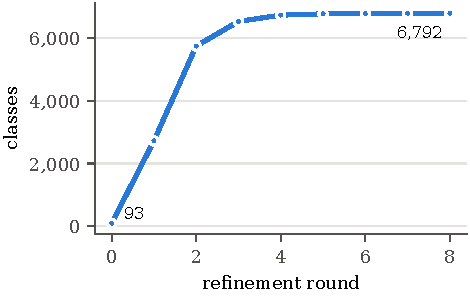
\includegraphics[width=0.48\linewidth]{figures/refinement.pdf}
\caption{Colour refinement from the radius-1 cut key.
Each round refines the previous partition (\cref{prop:refine}); the number of classes grows from 93 to 6{,}792 and then stops.
The 1{,}988 items left in shared classes are structurally indistinguishable at any depth.}
\label{fig:refinement}
\end{figure}

\paragraph{Ladders.}
The graph contains 17 maximal unbranched series chains.
The longest has ten rungs: the steps of retroviral reverse transcription, from RNase H cleavage of the RNA strand to synthesis of full-length duplex DNA.
Every chain's rung powers are \vd{absent}, with the blocker ``rung power needs junction conductances'': without conductances, \cref{prop:ladder} cannot be evaluated.

\subsection{Thermodynamic coverage}
\label{sec:res-thermo}

TECRDB contributes 418 reactions in the temperature and grade window, 295 of them with a transformed value in the pH window.
Matching gives 75 kernel reactions with a measured $\DG$, all via \conv{conjugate-closure} (71), a candidate selected by the TECRDB match (3) or water balance (1).
They correspond to 61 distinct TECRDB reactions.
Of the rest, 2{,}244 are \vd{refused} because a participant is a macromolecule, and 595 are \vd{absent}.
Of the absent, 398 have no TECRDB measurement and 197 have a participant without a KEGG identifier (\cref{fig:coverage}).

\begin{figure}[t]
\centering
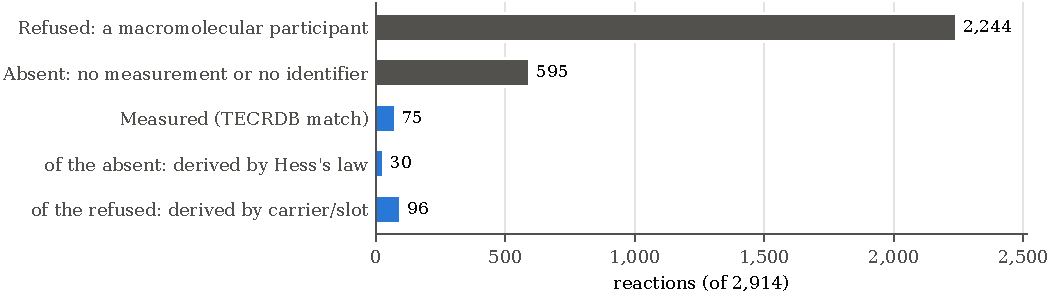
\includegraphics[width=0.85\linewidth]{figures/coverage.pdf}
\caption{Thermodynamic verdicts for the 2{,}914 cytosolic reactions.
Grey bars partition the reactions that TECRDB does not determine directly; blue bars are the reactions with a chemical-reference $\DG$.
Hess's law recovers 30 of the absent and the carrier/slot decomposition 96 of the refused.}
\label{fig:coverage}
\end{figure}

\paragraph{Cycle consistency.}
The 61 distinct matched reactions are linearly independent: $\ker S$ is trivial, and the cycle test is \vd{certified-empty}.
The question is well posed and its answer is empty, because the kernel's measured reactions close no cycle.
The full TECRDB set is not internally consistent.
The weighted Hess fit over 418 reactions and 495 compounds has $\chi^2=275.6$ on 67 degrees of freedom ($\chi^2/\nu=4.11$, Birge ratio 2.03), so the quoted uncertainties are about half the scatter they must explain.

\paragraph{Hess's law.}
Of 398 small-molecule reactions that TECRDB never measured directly, 30 lie in the span of the measured reactions and are \vd{answered} (\cref{prop:hess}).
One is \vd{certified-empty} (no net chemical change).
The other 367 are \vd{absent}: 324 contain a compound never measured in any TECRDB reaction, and 43 are not combinations of measured reactions.

\paragraph{Carrier and slot.}
Of the 2{,}244 refused reactions, 1{,}591 are not carrier reactions, because the protein entity differs between the two sides.
Of the remaining 653, 96 are \vd{answered} (94 kinase and 2 phosphatase steps) and 104 are \vd{underdetermined}, because the species names state a number of changed sites that does not match the number of kinase or phosphatase steps.
The other 453 are \vd{absent}: 373 involve carrier chemistry other than phosphoryl transfer, and 80 a compound that TECRDB never measured.

\paragraph{Enzyme expansion.}
Expanding the 1{,}116 catalysts into two-rung cycles gives 4{,}546 junctions over 6{,}962 species, with rank 4{,}299.
The conservation-law dimension stays 2{,}663 and the flux-mode dimension 247, as \cref{prop:enzyme} requires of an expansion that leaves net stoichiometries unchanged.
The enzyme total is conserved for 682 catalysts and broken for 434, which the stoichiometry also makes, consumes or modifies.

\paragraph{Direction in the base stage.}
With TECRDB's transformed study means in the pH window and the 1\,\textmu M--10\,mM concentration window, 3 reactions are \vd{answered} forward and 61 are \vd{undecidable}.
The remainder inherit \vd{absent} (606) or \vd{refused} (2{,}244) from the match.

\subsection{Proteins and attachment}
\label{sec:res-proteins}

Of the phosphosites named on carrier reactions, 206 were located in their protein's sequence with the named residue type.
Another 69 named no position, 9 named a residue type that differs from the sequence, 12 belong to proteins without an AlphaFold contact graph and 35 to an entity whose protein was not determined.
The located sites lie on 131 reactions and 101 proteins; attaching them adds 60{,}657 residue vertices, 222{,}072 contact edges and 206 slot edges.

\paragraph{Monotonicity and its control.}
Over the 60 items whose global separation cost was computed before and after attachment, attachment never lowered $\sigma$ (0 decreases, 20 increases), as \cref{prop:monotone} requires.
The control replaced each carrier--junction edge's counted weight by the slot residue's relative exposure, a real number in $(0,1]$.
It lowered $\sigma$ for 46 of the 60 items and raised it for 4, and the minimum fell from 2 to 1.14.
Local separation costs at radii 1 and 2 behave the same way under attachment: of 423 items, none decreased and 131 increased.

\paragraph{Exposure of phosphosites.}
Named sites are more exposed than residues of the same type in the same proteins (one-sided Mann--Whitney $p=0.0049$; 165 sites against 4{,}443 residues).
The medians are equal (5 exposed heavy atoms each), and the difference is at the bottom of the distribution: no named site is buried, against 3.1\% of the comparison residues.

\subsection{The medium as eluent (M1--M3)}
\label{sec:res-medium}

\paragraph{The transform.}
Our Legendre transform reproduces eQuilibrator's own transform on all 3{,}276 TECRDB rows in the window, with a largest difference of $6.8\times10^{-13}\kJ$.
Two controls confirm that the comparison can fail: shifting the pH by 0.1 leaves only 66 rows within $10^{-6}\kJ$, and dropping the Debye--H\"uckel term leaves 59.

\paragraph{M1: the medium transfers (supported).}
For TECRDB reactions measured under three or more distinct conditions, each condition was held out in turn and predicted from the others.
The \emph{medium} model fits one chemical-reference value per reaction and adds the held-out row's transform.
The \emph{constant} model predicts the training mean, and the \emph{affine-pH} model fits a line in pH (two parameters).
Replicate noise, the same reaction under the same conditions in different studies, is 1.38\kJ\ in mean (0.71 median) over 171 pairs.
\Cref{fig:transfer} gives the errors.
Paired per reaction, the medium model beats the constant model in 84 of 137 interpolated reactions (Wilcoxon $p=8\times10^{-4}$) and in 95 of 154 extrapolated ones ($p=5\times10^{-6}$).
Where the held-out transform moved by more than 1\kJ, the interpolation errors are 1.95 against 2.94\kJ; where it moved less, they are equal (1.08 and 1.08).
The medium model's mean error is 1.13 times the replicate noise in interpolation and 1.88 times in extrapolation, within the stated limit of twice the noise.
In extrapolation it is no worse than affine-pH (82 against 72 reactions, $p=0.27$).
One result was not predicted: in interpolation, the two-parameter affine-pH model beats the one-parameter medium model (77 against 58 reactions, $p=0.009$).

\begin{figure}[t]
\centering
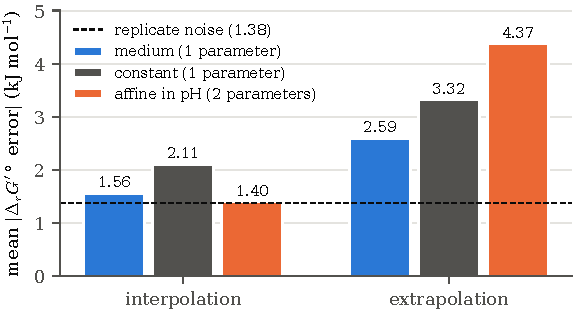
\includegraphics[width=0.62\linewidth]{figures/transfer.pdf}
\caption{Held-out prediction of transformed Gibbs energies (M1).
Mean absolute error over held-out TECRDB rows for three models.
The dashed line is the replicate noise between studies of the same reaction under the same conditions.}
\label{fig:transfer}
\end{figure}

\paragraph{M2: direction (count fails, attribution holds).}
Of the 201 reactions with a chemical value, 2 are \vd{answered} forward: pyrophosphate hydrolysis by the two cytosolic pyrophosphatases.
The claim of more than three answered fails.
The base stage's three answers used study means without uncertainty or ionic-strength and magnesium ranges.
Adding $q\sigma$ and those ranges removes one of them, AMP hydrolysis by a nucleotidase, which rested on a single study.
The two survivors clear zero by only 0.28\kJ.
The second part holds: of the 199 undecided reactions, 156 (78\%) have a fixed sign of $\DGm$ across the medium window, including all 96 carrier/slot reactions.
For these, the concentrations, not the medium, are what remain to be measured; the other 43 are blocked by the medium window itself.

\paragraph{M3: crowding and dilution (both fail).}
Crowding changes both of the two decided verdicts, far above the stated limit of 5\%.
In each pyrophosphate hydrolysis, one pyrophosphate and one water give two phosphates, so with water excluded the reaction adds one solute particle.
Its 0.28\kJ\ margin is below the 0.92\kJ\ crowding shift at $a=0.7$.
With crowding in the medium, no reaction in the kernel has a decided direction.
The dilute-solution bound $2nv$, with $n$ the number density at 10\,mM and $v$ the molecular volume, has a median of 0.0035 per particle but exceeds $10^{-2}$ for large compounds.
The worst is a 1{,}873\,Da compound (KEGG C05893) at 0.027.
The ideal-solution form of $\mu$ is safe for ordinary metabolites at 10\,mM, but not for molecules of this size at the top of the window.
A hard-sphere second-virial estimate would give a larger factor than $2nv$, which would strengthen this failure rather than remove it.

\subsection{Kinetics: retention, locality and K1}
\label{sec:res-kinetics}

SABIO-RK's 7{,}458 human wild-type entries with $K_m$ give 5{,}682 substrate $K_m$ records over 3{,}559 (protein, compound) pairs.

\paragraph{Retention.}
370 of the 1{,}631 catalysed kernel reactions have a measured $K_m$ for a substrate, giving 596 contacts.
Of 168 metabolites with a $K_m$, 161 have a PaxDb abundance for every binding enzyme.
Their median retention factor at total enzyme is 0.001--0.003 across the 2--6\,mM range of total protein, so metabolites are almost entirely free and binding barely raises their capacitance.
Only 8 exceed $k=1$ at the upper total, among them 5-diphosphoinositol pentakisphosphate ($k=9$--26), S-adenosylmethionine, fructose 1,6-bisphosphate and NADPH.

\paragraph{Locality.}
The enzymes are not dilute.
Over 223 enzymes, the median concentration $c^\ast$ at which the readout departs by 10\% from the dilute limit is 2.4\,\textmu M of substrate.
Of these enzymes, 76 depart below 1\,\textmu M of substrate.
None stays dilute across the whole concentration window, and 221 depart by more than 10\% at 1\,mM.
106 enzymes have two or more measured substrates that share the same sites.
In chromatographic terms the cytosolic column is overloaded.
For the metabolite the stationary phase is negligible ($k\ll1$), but for the enzyme the contacts are non-local (Langmuir rather than linear).
Enzyme--substrate states therefore cannot be folded into the free species' capacitance; they must stay explicit with conserved enzyme totals, as in \cref{sec:enzyme}.

\paragraph{K1: whole-protein descriptors do not carry $K_m$ (holds).}
Under leave-one-protein-out cross-validation over 272 proteins and 1{,}228 pairs, the baseline predicts each $K_m$ from the substrate's mean $\log_{10}K_m$ over other proteins.
The alternative adds a ridge map from five AlphaFold descriptors to the residual: residue count, mean pLDDT, fraction of buried residues, mean contact weight per residue and exposed atoms per residue.
Its ridge penalty is chosen by inner five-fold cross-validation.
The mean absolute errors are 0.775 and 0.780 $\log_{10}$ units.
The descriptor model is better for 105 proteins and worse for 127 (one-sided Wilcoxon $p=0.94$), so the claim that descriptors do not help holds.
The positive control adds a synthetic effect of 0.5 standard deviations of $\log_{10}$(residue count) to $\log_{10}K_m$; the test detects it ($p=0.007$), so it could have found an effect that the descriptors carry.

\subsection{Completion and separation}
\label{sec:res-complete}

The survey asks, for 540 small-molecule sources and 779 targets (420{,}120 pairs), whether the kernel turns the source into the target using only the source, the medium and the 2{,}241 proteins that no reaction makes.
\Cref{fig:completion} gives the outcomes under the three direction semantics.

\begin{figure}[t]
\centering
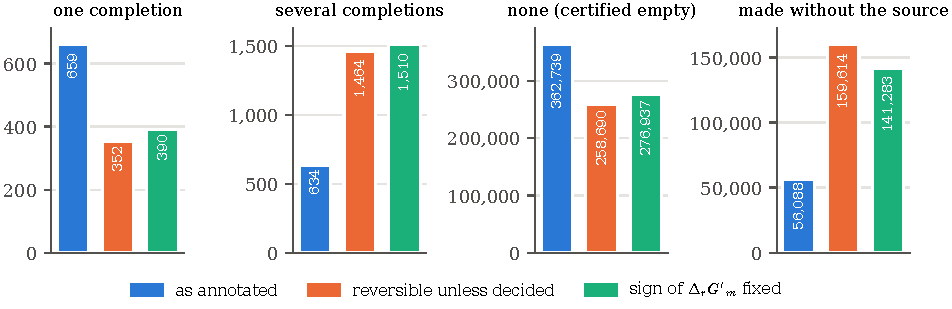
\includegraphics[width=\linewidth]{figures/completion.pdf}
\caption{Completion outcomes for 420{,}120 source--target pairs under three direction semantics.
Each panel has its own scale.
``Made without the source'' means the target is reached from the medium and proteins alone.}
\label{fig:completion}
\end{figure}

Most pairs have no completion, because most reactions need a second small molecule that a single source cannot supply.
Allowing reactions to run backwards halves the unique completions, from 659 to 352.
It also lets the medium and proteins make many more targets on their own (56{,}088 to 159{,}614).
Fixing the 158 directions whose $\DGm$ sign is fixed (two by measurement and 156 by the 1\,mM sign) adds 38 unique completions (+11\%) and removes 18{,}331 pairs from ``made without the source''.
A completion may not pass through its own target, but alternatives through other cycles among intermediates still count as several, so that column is an upper count.

\subsection{A coupled-oscillator account of folding (F1--F5)}
\label{sec:res-folding}

We tested an account of folding in which residues are phase oscillators coupled by a matrix $K$, secondary structure emerges as groups of phase-locked residues, and the number of large eigenvalues of $K$ counts secondary-structure elements.
The account is a variant of Kuramoto synchronisation \citep{kuramoto1984chemical} and is motivated by Levinthal's argument that folding cannot be an unbiased search \citep{levinthal1969fold,dill2012folding}.
Its coupling is built from sequence alone ($K_{\mathrm{seq}}$).
We also ran every test with the AlphaFold contact graph as coupling ($K_{\mathrm{AF}}$, counted heavy-atom pairs within 4.5\,\AA), which gives the account the real structure to work with.
Secondary-structure elements come from a backbone hydrogen-bond assignment in the manner of \citet{kabsch1983dssp}.
Against the authors' helix and sheet records in four experimental structures, that assignment agrees per residue at 0.87 (1CRN), 0.83 (1UBQ), 0.87 (2LZM) and 0.91 (3CHY), against 0.24--0.42 for shuffled residues.

\paragraph{F1: contacts from sequence (reproduction).}
On 607 AlphaFold models with mean pLDDT at least 90 and 50--400 residues, $K_{\mathrm{seq}}$ reaches a top-$L$ contact precision of 0.81 times the base rate, worse than random (two-sided Wilcoxon $p=7\times10^{-11}$).
A plain hydrophobicity product reaches 2.36 times the base rate.
No protein meets a criterion of precision at least 0.7 and recall at least 0.5 with either score.

\paragraph{F2: eigenvalue count equals the number of elements (fails).}
On 149 proteins with a median of 12 elements, no protein's count of $K_{\mathrm{seq}}$ eigenvalues above the threshold matches exactly, with a mean absolute error of 7.1; $K_{\mathrm{AF}}$ matches 3, with error 9.1.
A baseline that predicts the count from length alone matches 23, with error 2.2.
Both couplings give too many eigenvalues above threshold (medians 18 and 20), even $K_{\mathrm{AF}}$, which is built from the real structure.

\paragraph{F3: phase-lock groups are secondary structure (fails).}
Agreement with the element/loop segmentation, as the best adjusted Rand index over a sweep of coupling strengths, is 0.067 for $K_{\mathrm{AF}}$ phase-lock groups.
Equal contiguous blocks score 0.486 and win for 148 of 149 proteins.
$K_{\mathrm{seq}}$ groups score 0.001.
The dynamics also add nothing to the coupling they run on: the connected components of the top $K_{\mathrm{AF}}$ pairs score 0.057, and the dynamics win 80 proteins and lose 66 ($p=0.14$).

\paragraph{F4: phosphosites are less synchronised, and disorder accounts for it (both parts hold, the second weakly).}
Kuramoto dynamics on $K_{\mathrm{AF}}$ at a coupling of 2, fixed in advance, give each residue a local order parameter.
Over 158 located sites against 3{,}870 same-type residues, sites have lower local order (median 0.912 against 0.936, one-sided $p=0.012$) and lower pLDDT (53.7 against 57.9, $p=0.043$).
Within pLDDT strata the difference is not significant: $p=0.39$ below 70 (106 sites) and $p=0.13$ at 70 or above (52 sites).
The second part rests on an absence of significance in a small stratum whose medians still point the same way (0.933 against 0.953), so a small residual effect is not excluded.
D1 (\cref{sec:res-db}) returns to this with measured disorder.

\paragraph{F5: hierarchical ternary addresses (measurement).}
C$\alpha$ coordinates normalised to each protein's bounding cube were given interleaved base-3 addresses.
On 150 models, the distance-preservation bound holds for all 2{,}480{,}054 C$\alpha$ pairs.
The deepest level whose cells are at least 8\,\AA\ on a side is one full triple of digits (27 cells), and only 54.6\% of the 122{,}559 C$\alpha$ contacts share that prefix.
The address bounds distance when prefixes agree but misses 45\% of contacts that straddle a cell boundary; it is usable as a proximity key only together with neighbouring cells.

\subsection{Verdict axes and extensions (E1--E6)}
\label{sec:res-extend}

The extension stage used every human wild-type kinetic law in SABIO-RK, UniProt annotations for 3{,}207 proteins (1{,}481 with an EC number) and PaxDb abundances for 3{,}048 proteins.

\paragraph{E1: verdict axes (measurement).}
Every empty or absent verdict from the live producers carries a gate letter.
These producers are the thermodynamic match, Hess, carrier/slot, direction, modifiers, dividers, variants and the redox ladder.
Of 1{,}681 such verdicts, 686 are not recorded ($-$), 605 are a name the source never uses (\textsf{open}) and 390 are witnessed absent ($+$); none is undecided.
The ground verdicts of each fact family are those given in \cref{sec:ground}.
The stage digest is current under its own conventions and stale after a change of pH window.
On the specification example, \vd{subfloor} reproduces a composite of 0.9475 against a target of 0.95, a shortfall of 0.0025.
On real data, no ladder chain has all its rung conductances (0 of 17), so it never fires.

\paragraph{E2: modifiers (measurement).}
Of 175 inhibitor edges, 147 are macromolecular partners and \vd{refused}; 26 small molecules have no $K_i$ for their enzyme in SABIO-RK ($-$) and 2 have no KEGG compound (\textsf{open}).
Of 105 stimulator edges, 52 are macromolecular, and the 53 small molecules have no activation constant.
No modifier edge is answered.
The 434 broken enzyme totals arise from assembly or dissociation (266), covalent modification (140), degradation (124) and other reactions (103); an enzyme may have several kinds, and where only one applies the counts are 91, 52, 49 and 45.
Such reactions are the boundary currents through which induction and inactivation would act.
Of 58 loss-of-function variant reactions, 23 attach to a single wild-type edge as a modifier, 19 match several (\vd{underdetermined}) and 16 match none.

\paragraph{E3: flux dividers (measurement).}
Of 168 branch points in healthy cells, 3 are \vd{answered}; the others lack $k_{\mathrm{cat}}/K_m$ for a sibling (487 sibling gaps) or have an uncatalysed sibling (135).
On average 7.6\% of a branch point's siblings are complete.
The answered shares are: fructose 1,6-bisphosphate to fructose-1,6-bisphosphatase 0.67 and aldolase 0.33; galactose to galactokinase 0.98 and aldose reductase 0.02; glucose to aldose reductase 0.52 and hexokinases 0.48.
The glucose share is not credible.
At millimolar glucose the hexokinases are saturated ($K_m$ about 0.1\,mM), so the dilute limit does not hold; this repeats the locality failure of \cref{sec:res-kinetics}.

\paragraph{E4: the redox ladder (E4a, E4b hold; E4c untestable).}
\Cref{tab:redox} gives the couple potentials derived from the Hess span.
The NAD and NADP couples lie 1.6\,mV apart, within the predicted 10\,mV (E4a).
With glutathione disulfide (GSSG) and reduced glutathione (GSH), NADPH + GSSG $\to$ NADP$^+$ + 2\,GSH has $\DGp=-13.8\kJ$, inside the predicted $-16\pm10\kJ$ (E4b).
Cystine and dehydroascorbate were never measured in TECRDB (\textsf{open}), and flavin adenine dinucleotide is not a combination of measured reactions ($-$).
For E4c, the flavin-to-cysteine edge distance is 3.42\,\AA\ in glutathione reductase (Protein Data Bank (PDB) entry 3GRS) and 3.33\,\AA\ in thioredoxin reductase 1 (2J3N).
Both give a ruler rate of $6.8\times10^{10}\,\mathrm{s^{-1}}$, and the control at 25\,\AA\ gives $0.014\,\mathrm{s^{-1}}$, so the check could discriminate.
SABIO-RK has no human wild-type $k_{\mathrm{cat}}$ for either enzyme, so E4c is \vd{absent} and untested.

\begin{table}[t]
\centering
\caption{Redox couples derived from the Hess span at pH 7, $I=0.25$\,M, 298.15\,K, relative to NADP$^+$/NADPH.
Textbook differences are approximate.}
\label{tab:redox}
\small
\begin{tabular}{@{}lrrr@{}}
\toprule
Couple & $E-E_{\mathrm{NADP}}$ (mV) & $\sigma$ (mV) & Textbook difference (mV) \\
\midrule
NAD$^+$/NADH & $+1.6$ & 7.5 & $+4$ \\
GSSG/GSH & $+71.7$ & 12.7 & about $+84$ \\
lipoamide & $+25.1$ & 29.1 & about $+34$ \\
thioredoxin & $+57.9$ & 28.2 & about $+54$ \\
pyruvate/lactate & $+138.7$ & 10.6 & $+139$ \\
oxaloacetate/malate & $+156.6$ & 9.1 & $+158$ \\
\bottomrule
\end{tabular}
\end{table}

\paragraph{E5: EC labels are concordant with structural classes (holds).}
Real level-1 EC labels split 4 of the 147 shared junction classes that carry labels (210 labelled junctions).
Shuffled labels split 53.7 on average, with a minimum of 41 (empirical $p=0.005$); at level 3 the counts are 4 against 61.8.
For 100 classes no label splits them (\vd{underdetermined}).
For the rest, the coarsest splitting label is the gene (18), EC level 1 (11), Pfam (8), EC level 4 (8), EC level 2 (1) or EC level 3 (1), and 32 classes are separated completely.
The bits left per item fall from 0.649 with structure alone to 0.641 with EC level 1, 0.629 with EC level 4, 0.627 with Pfam and 0.619 with the gene.

\paragraph{E6: stoichiometric signatures match EC classes (holds).}
The signature rules give 798 \vd{answered}, 42 \vd{underdetermined} (28 of them lyase and transferase together), 653 \vd{absent} and 1{,}421 \vd{refused} verdicts.
On 634 reactions with a single-class catalyst, the signature agrees with the EC class in 593 (93.5\%), against 32.5\% for shuffled labels (empirical $p=0.005$).
The largest confusions are lyase against EC oxidoreductase (8) and hydrolase against EC transferase (8).

\subsection{Cross-checks against curated databases (R1--G1)}
\label{sec:res-db}

\paragraph{R1: curated direction against the 1\,mM sign (fails).}
460 kernel reactions map to Rhea (403 left-to-right, 69 right-to-left), and their participant sets agree in 421 of 459.
For the 62 mapped reactions whose $\DGm$ sign is fixed across the medium window, the sign agrees with the curated direction in 45 (72.6\%), below the predicted 80\%.
The 17 disagreements are not errors of sign.
They include triose-phosphate isomerase, glyceraldehyde-3-phosphate dehydrogenase, lactate oxidation by lactate dehydrogenase, ethanol oxidation, creatine kinase forming phosphocreatine and the thiolase condensation of two acetyl-CoA.
All of them run uphill at 1\,mM and proceed in the cell because product is drawn away.
The 1\,mM sign is not a direction; the concentration ratio is.
Measured concentration windows (\cref{sec:loaders}) would decide exactly these reactions.

\paragraph{I1: MetaNetX closes identifier misses (fails).}
MetaNetX gives 36 more species a KEGG compound and unblocks 34 of the 197 reactions blocked by a missing identifier (17\%, against a predicted quarter).
One of them gains a TECRDB match, and 33 are now blocked by ``no TECRDB measurement of this reaction''; the Hess-derived count stays at 30.
The gate letter of those 33 changes from \textsf{open} to $-$: the limit is measurement, not identifiers.

\paragraph{L1: catalysts have cytosol support (holds).}
Of 2{,}134 catalyst proteins, 1{,}947 have cytosol support, 100 have none and 87 have no data, so 95.1\% of those with data are supported.
By reaction, 1{,}404 have all catalysts supported, 79 some and 78 none.
The unsupported proteins include the three fibrinogen chains (UniProt P02671, P02675 and P02679), which are secreted.
The 78 reactions are candidates for errors in the cytosol annotation from which the corpus was filtered.

\paragraph{S1: slots sit on curated phospho-residues (holds).}
168 of the 206 located phosphosites (81.6\%) coincide with a UniProt phospho modified residue.
141 of the 168 carry experimental evidence (ECO:0000269 or ECO:0007744).
One numbering offset per protein explains 5 of the 9 residue mismatches: $+39$ in Q04637 (3 sites), $+2$ in Q14155 and $-48$ in tau (P10636, an isoform numbering).
UniProt also names 31 phosphorylated enzyme intermediates (phosphohistidine, phosphocysteine, phosphoserine) among the catalysts; these are the enzymes whose two-rung expansion should carry a covalent intermediate.
A first run reported 19\%: the parser cut each UniProt note at its first semicolon, losing notes such as ``Phosphoserine; by MTOR'' that name the kinase, here the mechanistic target of rapamycin (MTOR).
The corrected parser has a regression test.

\paragraph{C1: catalytic residues are contact hubs (holds).}
Over 50 M-CSA enzymes, 255 catalytic residues have a median of 55 heavy-atom contacts, against 43 for the 3{,}773 residues of the same amino-acid types in the same AlphaFold models (one-sided Mann--Whitney $p=2.7\times10^{-18}$).
A random same-type sample of equal size gives $p=0.46$.

\paragraph{A1: AlphaFold contacts match experiment (holds).}
Of 313 high-confidence models, 60 were compared with an experimental chain (\cref{fig:structures}).
The median Jaccard index of contact sets is 0.90; shifting one numbering by three residues drops it to 0.14.
Buried and exposed calls agree for 95\% of residues.
On these proteins, the AlphaFold contact graphs used for attachment and for F1--F5 stand in for measured ones.

\begin{figure}[t]
\centering
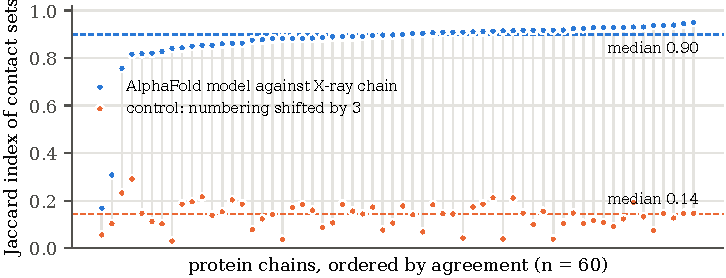
\includegraphics[width=0.85\linewidth]{figures/structures.pdf}
\caption{Contact agreement between AlphaFold models and X-ray chains for 60 proteins (A1).
Blue: Jaccard index of residue contact sets.
Orange: the same after shifting one numbering by three residues.
Dashed lines are medians.}
\label{fig:structures}
\end{figure}

\paragraph{D1: measured disorder explains the phosphosite effect (fails).}
Over 40 proteins with located sites and DisProt entries, named sites outside the disordered regions still have lower local order than same-type residues (median 0.88 against 0.94, one-sided $p=0.0012$, 34 sites).
Inside disordered regions they do not differ ($p=0.37$, 26 sites).
Measured disorder does not account for the effect that pLDDT appeared to account for in F4.
DisProt is incomplete, so ``outside a DisProt region'' is not the same as ``ordered''.

\paragraph{G1: Human-GEM coefficients agree (holds, weakly discriminating).}
505 kernel small-molecule reactions have KEGG identifiers for every participant; 324 match a Human-GEM cytosolic reaction by participant set, and all 324 have the same coefficients.
Only 23 of them have a coefficient other than 1, so the agreement rests on those 23.
Reversibility agrees in 244 of 324.

\paragraph{Per-cell-type abundance.}
With HeLa abundances \citep{nagaraj2011hela} in place of whole-organism ones, 1 branch point is answered instead of 3; galactose goes to galactokinase with share 0.96, against 0.98.

\subsection{Summary of outcomes}
\label{sec:res-summary}

\Cref{tab:outcomes} lists the 23 pre-registered claims.
Fourteen held, eight failed and one could not be tested.

\begin{table}[p]
\centering
\caption{Outcomes of the 23 pre-registered claims.}
\label{tab:outcomes}
\small
\begin{tabularx}{\linewidth}{@{}l>{\raggedright\arraybackslash}Xl>{\raggedright\arraybackslash}p{4.6cm}@{}}
\toprule
ID & Claim & Outcome & Key number \\
\midrule
M1 & the medium transform transfers between conditions & holds & error 1.13$\times$ (interp.) and 1.88$\times$ (extrap.) replicate noise \\
M2a & more than 3 reactions get a direction & fails & 2 answered \\
M2b & concentrations, not the medium, block most of the rest & holds & 156 of 199 \\
M3a & crowding changes at most 5\% of decided verdicts & fails & 2 of 2 changed \\
M3b & dilute bound below $10^{-2}$ for every metabolite at 10\,mM & fails & worst 0.027 \\
K1 & protein descriptors do not improve $K_m$ prediction & holds & $p=0.94$; positive control $p=0.007$ \\
F2 & eigenvalue count equals number of elements & fails & 0 and 3 exact, against 23 for length \\
F3 & phase-lock groups beat contiguous blocks & fails & 0.067 against 0.486 \\
F4a & phosphosites have lower local order & holds & $p=0.012$ \\
F4b & no difference within pLDDT strata & holds (weak) & $p=0.39$ and $0.13$ \\
E4a & NAD and NADP couples within 10\,mV & holds & 1.6\,mV \\
E4b & NADPH reduces GSSG, $\DGp$ within $-16\pm10\kJ$ & holds & $-13.8\kJ$ \\
E4c & ruler rate exceeds $k_{\mathrm{cat}}$ & untestable & no $k_{\mathrm{cat}}$ in SABIO-RK \\
E5 & EC labels split fewer classes than shuffled labels & holds & 4 against 53.7; $p=0.005$ \\
E6 & signatures agree with EC classes above 60\% and the null & holds & 93.5\% against 32.5\% \\
R1 & 1\,mM sign agrees with curated direction above 80\% & fails & 72.6\% \\
I1 & MetaNetX unblocks at least a quarter of 197 reactions & fails & 34 (17\%) \\
L1 & at least 80\% of catalysts have cytosol support & holds & 95.1\% \\
S1 & at least 70\% of slots on phospho-residues; offsets explain a third of mismatches & holds & 81.6\%; 5 of 9 \\
C1 & catalytic residues have more contacts & holds & $p=2.7\times10^{-18}$; control $p=0.46$ \\
A1 & median contact Jaccard at least 0.6; shifted control below 0.2 & holds & 0.90; 0.14 \\
D1 & outside DisProt disorder, sites do not have lower order & fails & $p=0.0012$ \\
G1 & Human-GEM coefficients agree in at least 90\% & holds & 324 of 324 (23 discriminating) \\
\bottomrule
\end{tabularx}
\end{table}

%==============================================================================
\section{Discussion}
\label{sec:discussion}

\subsection{What typed verdicts buy}
\label{sec:disc-verdicts}

An inference engine asked for the Gibbs energy of 2{,}914 cytosolic reactions returns 75 values and silence.
The kernel returns 2{,}914 verdicts, and the silence is resolved by cause.
For 2{,}244 reactions the question is outside what TECRDB can state; for 398 no measurement exists; for 197 the reaction cannot even be put to TECRDB, because a participant has no identifier it uses.
These three populations need different remedies.
The first needs a different kind of model, such as the carrier/slot decomposition, which recovered 96.
The second needs measurement or estimation.
The third needs cross-references, and I1 (\cref{sec:res-db}) shows how far those go: MetaNetX moved 33 reactions from the third population into the second and none into the answered set.
The gate letters made that movement visible as a change from \textsf{open} to $-$.

The payload rule (V1) did real work.
A missing $\DG$ never became zero, a missing $K_m$ never became a typical value, and an undecided direction never became the curated one.
Every downstream count in this paper, from 156 concentration-blocked directions to 3 answered branch points, inherits that discipline.
The rule also makes failures cheap to diagnose: the S1 parser fault surfaced as an implausibly low fraction rather than as silently wrong slot energies, because the slot check reads curated features directly.

Basis tags and ground verdicts answer a different question: not ``is there a value?'' but ``what kind of value is it?''.
The AlphaFold contact graphs are icons, models of their object; A1 shows that on 60 proteins they agree with indices, crystal structures, at a median Jaccard index of 0.90 (\cref{fig:structures}).
That agreement licenses using them where no crystal structure exists, but it does not turn them into measurements, and the ground verdict keeps saying so.
The falsifiability guard (\cref{prop:falsifiable}) is the same idea applied to cycles: a consistency check that cannot fail is refused, not passed.

\subsection{Concentrations are the binding constraint}
\label{sec:disc-conc}

Three independent results point to the same missing datum.
M2b found that for 156 of 199 undecided reactions the medium fixes the sign of $\DGm$, so only concentrations remain.
R1 found that the curated directions which disagree with the 1\,mM sign are those of reactions running uphill at 1\,mM, such as triose-phosphate isomerase and glyceraldehyde-3-phosphate dehydrogenase, which glycolysis pulls forward by removing product.
The completion survey found that fixing those directions adds 11\% more unique completions (\cref{sec:res-complete}).
Absolute concentrations measured in mammalian cells \citep{park2016concentrations} are therefore the single most valuable addition to the kernel.
The loader for them exists (\cref{sec:loaders}); its file does not yet.

The same result reframes what a ``direction'' annotation is.
A curated direction is a statement about the physiological concentration regime, not about the reaction.
The kernel's direction verdict makes the dependence explicit: its blocker names the concentration window, and its remedy names the measurement.

\subsection{Enzymes are not dilute}
\label{sec:disc-locality}

The chromatographic reading of the cytosol gives two numbers per contact, and they point in opposite directions.
From the metabolite's side, retention is negligible: the median $k$ is 0.001--0.003, so binding barely changes a metabolite's capacitance.
From the enzyme's side, contacts are non-local (\cref{sec:res-kinetics}): the median enzyme departs from its dilute limit at 2.4\,\textmu M of substrate, and 221 of 223 depart by more than 10\% at 1\,mM.
The consequence for modelling is concrete.
Enzyme--substrate states cannot be folded into metabolite capacitances; they must stay explicit, with conserved enzyme totals, which is what the two-rung expansion provides.
The failure of the glucose divider in E3 is the same fact seen from the flux side: shares computed in the dilute limit are wrong where the enzyme is saturated.

\subsection{What failed, and why that matters}
\label{sec:disc-negative}

The coupled-oscillator account of folding failed every test it could fail.
Its sequence coupling carries less contact information than a hydrophobicity product (F1).
Its eigenvalue count misses even with the true contact graph as coupling (F2).
Its phase-lock groups lose to contiguous blocks (F3), and its dynamics add nothing to the static coupling they run on ($p=0.14$).
F4 appeared to rescue a weak effect by attributing it to disorder, and D1 then removed the rescue, because the effect persists outside measured disordered regions.
The pattern argues against adopting the account as a structure source and for keeping AlphaFold's counted contact graph, whose agreement with experiment A1 established (\cref{fig:structures}).

M3 failed in an instructive way.
The two reactions whose direction the kernel decides clear zero by 0.28\kJ; a crowding shift of 0.92\kJ\ removes both.
A direction verdict that a plausible change of convention can overturn is not robust, and the kernel reports it as such.

G1 held, but only 23 of its 324 cases could have failed (\cref{sec:res-db}), and the paper says so.
A check is only as strong as its discriminating cases, which is why the check markers distinguish \emph{pass} from \emph{non-discriminating}.

\subsection{Limitations and threats to validity}
\label{sec:limitations}

\paragraph{Scope of the corpus.}
The corpus is defined by Reactome's compartment annotations.
L1 found 78 reactions none of whose catalysts has cytosol support, including secreted fibrinogen chains; these are likely annotation errors that the filter inherited.
Reactions that span compartments, including all transport, are excluded by construction.

\paragraph{Coverage of measured thermodynamics.}
Only 61 distinct TECRDB reactions match the corpus, and they close no cycle, so the cycle test is \vd{certified-empty} rather than informative.
The wider TECRDB set is inconsistent at $\chi^2/\nu=4.11$, so its quoted uncertainties are optimistic by a factor of about two.
The pooled $\sigma$ of 2.68\kJ\ is applied uniformly and does not capture reaction-specific error.

\paragraph{Conventions are supplied, not measured.}
The medium window, the concentration window, the ambient list, the conversion from parts per million to molar and the accessible-volume range are typical cytosolic values, not measurements for any cell type.
Each is named on every value it affects, and each enters the stage digest, but a different choice changes the numbers.
Abundances are whole-organism integrated values except in the HeLa comparison.

\paragraph{Temperature.}
Transforms are evaluated at 298.15\,K because TECRDB values are not temperature-corrected.
The concentration term of the direction verdict and the junction law use $RT$ at 310\,K (2.577\kJ).
The mismatch scales $RT\ln Q$ by about 4\%, and it is not negligible.
Evaluating the concentration term at 298.15\,K as well would decide eight further reactions forward.
All eight are cAMP hydrolysis by phosphodiesterases, with Hess-derived values, and they clear zero by 0.8\kJ.
Like the two pyrophosphatase verdicts, these sit within a convention's reach of the boundary.
A consistent treatment would correct the standard values to 310\,K before any of them is relied on.

\paragraph{Multiple testing.}
The 23 claims were tested at $\alpha=0.05$ without correction, as declared.
Most decisive outcomes are far from the threshold, for example C1 ($p=2.7\times10^{-18}$) and the shuffle tests ($p=0.005$, the smallest attainable with 200 permutations).
F4a ($p=0.012$) and the pLDDT difference within it ($p=0.043$) would not survive a Bonferroni correction over 23 claims, and should be read as suggestive.

\paragraph{Single runs and implementation faults.}
Each stage was run once on fixed data.
One implementation fault was found during the work and is reported with its effect: the UniProt parser initially truncated notes at semicolons, which lowered S1 from 81.6\% to 19\% until it was fixed.
The test suite (\cref{app:tests}) guards each such fault found so far, but it cannot exclude faults not yet found.

\paragraph{Missing data sources.}
Two sources the design anticipates could not be obtained under their terms.
The supplementary concentration tables of \citet{park2016concentrations} require a publisher login, and the Human Metabolome Database refused scripted downloads \citep{wishart2022hmdb}.
BRENDA requires a licence to be accepted interactively \citep{chang2021brenda}, and PhosphoSitePlus requires registration under a non-commercial licence \citep{hornbeck2015psp}.
Their loaders are in place, and their verdicts are \vd{absent} until the files are supplied.

%==============================================================================
\section{Conclusion}
\label{sec:conclusion}

A knowledge graph of biochemistry need not infer.
When its edges are element laws and its nodes are solutions, its structure yields rank, conservation laws, blocked reactions and cycle constraints without any parameter.
When its answers are typed verdicts with non-launderable provenance, every gap is named by cause, and every remedy is explicit.
Applied to the human cytosol, the kernel shows how little of the network public measurements determine (\cref{tab:outcomes,fig:coverage}): 201 of 2{,}914 reaction energies, 2 robust directions, 3 flux dividers.
It also shows precisely what would determine more (\cref{sec:disc-conc}).
Concentrations would decide most directions; measurement, not identifiers, limits thermodynamic coverage; enzyme saturation, not metabolite sequestration, governs the contacts.
The pre-registered audit kept the kernel honest about all of this, including the claims that failed.


\section*{Data and code availability}
The kernel is the Python package \texttt{circuit\_kg} (about 5{,}900 lines), on branch \texttt{circuit-kg} of the author's \texttt{nebuchadnezzar} repository.
The results reported here are from commit \texttt{15fb81a}.
The hypotheses were committed in \texttt{de6f210}, \texttt{d77d09c}, \texttt{cddf153} and \texttt{b1d7fc8}, each before the code that tested them.
Every downloaded file is recorded with its address, retrieval date and SHA-256 digest in \texttt{data/raw/SOURCES.json}.
Every number in this paper is read from \texttt{results/*.json}; the figures are drawn from those files by \texttt{paper/figures/make\_figures.py}.
The commands that regenerate each stage are listed in \cref{app:reproduce}.

\bibliographystyle{unsrtnat}
\bibliography{refs}

\appendix
%==============================================================================
\section{Named conventions}
\label{app:conventions}

Every supplied value names the convention that produced it.
\Cref{tab:conventions} lists them all.

{\small
\begin{longtable}{@{}>{\raggedright\ttfamily}p{5.3cm}>{\raggedright\arraybackslash}p{10.2cm}@{}}
\caption{Conventions supplied by the kernel.}\label{tab:conventions}\\
\toprule
\normalfont Convention & Meaning \\
\midrule
\endfirsthead
\toprule
\normalfont Convention & Meaning \\
\midrule
\endhead
\bottomrule
\endfoot
ambient-reservoir & the 14 cofactors of \cref{sec:medium-ground} are folded into the medium vertex \\
medium-floor & every item has a medium edge of weight 1 \\
modifier-unit-weight & every modifier edge has weight 1 \\
conjugate-closure & a KEGG compound reached through conjugate acids, conjugate bases and tautomers \\
water-balance & a TECRDB match that holds once water is balanced \\
concentration-window & 1\,\textmu M to 10\,mM for every metabolite \\
pH-window & pH 6.8 to 7.6 (base stage) \\
medium-window & pH 6.8--7.6, ionic strength 0.1--0.25\,M, pMg 2.8--3.5, 298.15\,K \\
accessible-volume & $\mu=\mu^\circ+RT\ln(c/a)$ with one $a\in[0.7,1]$ for every small solute \\
hess-span & a $\DG$ derived from measured reactions by Hess's law \\
carrier-slot & a protein that is the same on both sides of a reaction adds nothing to its $\DG$ \\
free-residue & a residue in a protein reacts like the free amino acid \\
slot-from-name & modified residues are read from Reactome species names \\
enzyme-cycle-2 & each catalysed reaction becomes a binding rung and a catalytic rung \\
medium-floor-residue & a buried residue still receives a medium edge of weight 1 \\
protein-ppm-to-molar & PaxDb parts per million times 2--6\,mM total protein molecules \\
scope-from-source & a completion may use the source, the medium and the proteins that no reaction makes \\
dilute-limit-share & a branch's share is $(k_{\mathrm{cat}}/K_m)[E]$ over the sum of its siblings', with $k_{\mathrm{cat}}$ paired to $K_m$ within one kinetic law \\
loss-of-function-variant & Reactome's ``Defective \dots'' reactions are modifiers on their wild-type edge \\
textbook-standard-conditions & redox couples at pH 7, ionic strength 0.25\,M, 298.15\,K, no magnesium \\
moser-dutton-defaults & reorganisation energy 0.7\,eV, driving force 0, packing density 0.76 \\
medium-as-slowest-rung & when a ladder's floor is judged, its medium resistance equals its slowest rung's \\
mnx-xref & a KEGG compound for a ChEBI accession reached through a MetaNetX identifier, only where \texttt{conjugate-closure} found none \\
measured-window & a per-compound concentration window from a declared table, replacing \texttt{concentration-window} for the compounds it lists \\
brenda-same-reference & a BRENDA $k_{\mathrm{cat}}$ is paired with a $K_m$ only for the same protein, substrate and reference \\
\end{longtable}}

%==============================================================================
\section{Test suite}
\label{app:tests}

The suite has 53 tests in eight files, and it passes in full at commit \texttt{15fb81a}.
Each test pairs an assertion with a control that must change the outcome, so a test that cannot fail would itself fail review.
\Cref{tab:tests} groups them by what they guard.

\begin{longtable}{@{}p{3.0cm}>{\raggedright\arraybackslash}p{11.6cm}@{}}
\caption{Tests and their controls.}\label{tab:tests}\\
\toprule
Area & Assertion (control) \\
\midrule
\endfirsthead
\toprule
Area & Assertion (control) \\
\midrule
\endhead
\bottomrule
\endfoot
Verdicts & a non-answered verdict cannot carry a payload; a non-answer must name its blocker (constructing a violating verdict raises) \\
Cut keys & cut keys are invariant under relabelling (changing a weight changes the key); $\sigma$ is intensive while the global floor version is not \\
Refinement & classes respect automorphism orbits, and each round refines the last (nodes outside an orbit are split) \\
Cycle test & consistent synthetic cycles pass and a planted defect is flagged; species-level errors cancel around cycles (\cref{prop:falsifiable}) \\
Ladders & rung powers telescope and shares equal flux control coefficients (\cref{prop:ladder}), checked against finite differences (shares differ when conductances differ) \\
Mass action & Gauss--Seidel relaxation matches the analytic steady state and detailed balance \\
Extraction & every kept reaction has every participant and modifier in the cytosol \\
Orientation & transformed TECRDB values are in the canonical orientation (triose-phosphate isomerase favours dihydroxyacetone phosphate on both scales) \\
Rank & the rank cut keeps small genuine singular values (a size-scaled cut invents null vectors) \\
Hess & a combination of measured reactions is recovered, and a target outside the span is refused \\
Slots & site parser formats and slot reactions (a name such as ``p-AMPK heterotrimer'' is not a site; one ATP for two named sites is underdetermined) \\
Enzymes & the two-rung expansion conserves the enzyme total and keeps net stoichiometry \\
Attachment & expansion never lowers global $\sigma$, but replacement by real-valued weights can \\
Surface area & vectorised Shrake--Rupley matches brute force and the isolated-sphere area \\
Medium & the transform reproduces eQuilibrator, and a perturbed transform does not; the transfer test rewards a correct transform and not a wrong one; crowding shifts only reactions that change particle number \\
Kinetics & $K_m$ records keep wild-type molar substrate constants only; locality labels follow the dilute threshold; K1 finds a planted descriptor effect and not a missing one \\
Completion & a chain is answered, a branch underdetermined and a missing co-substrate empty; direction constraints change completions; targets made without the source are set aside \\
Folding & vectorised coupling equals the reference loop; identical coupled oscillators lock and detuned uncoupled ones do not; segmentation gives one group per element and per loop stretch; the ternary address is a bijection whose bound holds and whose converse fails; the secondary-structure assignment matches author records and shuffling breaks it \\
Verdict axes & basis composes as a maximum with absent dominating; gate letters only on empty or absent verdicts; ground verdicts follow the provenance chain; a stage is invalidated by a convention change; \vd{subfloor} names its shortfall; a check whose control passes is non-discriminating \\
Extensions & inhibitor shift and absent stack; variants attach to their wild-type edge; divider shares follow specificity times amount and name missing siblings; $k_{\mathrm{cat}}$ pairs with the $K_m$ of the same kinetic law; the Moser--Dutton rate decays with distance; concordant labels split fewer classes than shuffled ones; stoichiometric signatures \\
Databases & \emph{estimated} is its own basis and ground; the falsifiability guard refuses derived-only cycles (one measurement lifts it); the Human-GEM comparison detects a coefficient difference; MetaNetX rescue fills only species without KEGG; scope check counts support; UniProt features parse and offsets are found (no offset for an absent residue type); feature notes may contain semicolons; a contact shift breaks agreement; measured windows decide a direction the global window cannot; BRENDA pairs need a shared reference \\
\end{longtable}

%==============================================================================
\section{Reproduction}
\label{app:reproduce}

From the repository root, the stages run in order:
\begin{center}
\begin{tabular}{@{}>{\ttfamily}l>{\raggedright\arraybackslash}p{8.2cm}@{}}
\toprule
\normalfont Command & Output and time \\
\midrule
python -m circuit\_kg fetch & ChEBI flat files (about 14\,MB) and the TECRDB table \\
python -m circuit\_kg extract & cytosolic corpus, about 100\,s \\
python -m circuit\_kg build & \texttt{summary.json}, \texttt{graph.json}, \texttt{supplements.json}; about 13\,min \\
python -m circuit\_kg proteins & AlphaFold residue contact graphs \\
python -m circuit\_kg attach & \texttt{attach.json} \\
python -m circuit\_kg medium & \texttt{medium.json}; about 30\,s \\
python -m circuit\_kg kinetics & \texttt{kinetics.json}; about 5\,min \\
python -m circuit\_kg complete & \texttt{complete.json}; about 45\,s \\
python -m circuit\_kg folding & \texttt{folding.json}; about 15\,min \\
python -m circuit\_kg extend & \texttt{extend.json}; about 1\,min \\
python -m circuit\_kg databases & \texttt{databases.json}; about 12\,min \\
python -m pytest circuit\_kg/tests -q & 53 tests, about 3\,min \\
\bottomrule
\end{tabular}
\end{center}
Most of \texttt{build}'s time is the singular value decompositions of the stoichiometric matrix before and after enzyme expansion.
The \texttt{medium} stage reads the local eQuilibrator compound cache.
The first run of each network-dependent stage downloads and caches its sources; later runs read the caches.

%==============================================================================
\section{Text of the claims}
\label{app:claims}

The claims are given here as recorded, with identifiers mapped as in \cref{tab:ids}.
Each states what would count against it.

\begin{description}[style=nextline,leftmargin=1.2cm,itemsep=3pt]
\item[M1] On TECRDB reactions measured under three or more distinct conditions, hold out one condition at a time.
The medium model's mean absolute error approaches the replicate noise and is below the constant model's, with the largest advantage where the held-out transform moved by more than 1\kJ.
In extrapolation it is no worse than affine-pH.
\emph{Against:} error above twice the replicate noise; no advantage where the medium moved; or affine-pH better in extrapolation.
\item[M2] More than the base stage's 3 reactions get a direction (M2a).
For most of the rest the sign of $\DGm$ is fixed across the medium window, so the blocker is the concentration window (M2b).
\emph{Against:} for most reactions the medium window alone admits both signs.
\item[M3] Crowding with $a\in[0.7,1]$ changes at most a few direction verdicts (M3a).
The dilute-solution bound stays below $10^{-2}$ per particle for every metabolite at 10\,mM (M3b).
\emph{Against:} crowding changes more than 5\% of decided verdicts, or the bound exceeds $10^{-2}$ for any metabolite.
\item[K1] Under leave-one-protein-out, a ridge map from five AlphaFold descriptors does not reduce the error of a substrate baseline for $\log_{10}K_m$ (one-sided Wilcoxon $p\ge0.05$).
\emph{Against:} $p<0.05$ with lower mean error.
\item[F2] The number of eigenvalues of $K$ above $\lambda_c=K_0e^{-1/2}\bar L$ equals the number of secondary-structure elements.
\emph{Against:} exact-match rate no higher than a length-only baseline.
\item[F3] Phase-lock groups from $K_{\mathrm{AF}}$ beat equal contiguous blocks per protein (one-sided Wilcoxon $p<0.05$).
\emph{Against:} $p\ge0.05$.
\item[F4] Named sites have lower local order than same-type residues (F4a); within pLDDT strata below 70 and at least 70 the difference has one-sided Mann--Whitney $p\ge0.05$ (F4b).
\emph{Against:} F4a has $p\ge0.05$, or F4b fails.
\item[E4a] NAD$^+$/NADH and NADP$^+$/NADPH lie within 10\,mV of each other.
\item[E4b] $\DGp$ of NADPH + GSSG $\to$ NADP$^+$ + 2\,GSH is negative and within 10\kJ\ of $-16\kJ$.
\item[E4c] For glutathione reductase and thioredoxin reductase 1, the ruler rate from the flavin-to-cysteine edge distance exceeds the measured $k_{\mathrm{cat}}$; the control at 25\,\AA\ falls below it.
A value that cannot be derived is recorded as \vd{absent}, not as a failure.
\item[E5] Real EC labels split fewer shared classes than labels shuffled among the same junctions (200 shuffles, empirical $p<0.05$).
\item[E6] On reactions whose catalyst has a single EC class, the signature class agrees with it in more than 60\% of classifiable reactions and above a shuffle null ($p<0.05$).
\item[R1] For reactions mapped to a directional Rhea reaction, the fixed sign of $\DGm$ agrees with Rhea's direction in more than 80\%.
\item[I1] MetaNetX supplies a KEGG compound for a participant in at least a quarter of the 197 reactions blocked by a missing identifier.
\item[L1] At least 80\% of catalyst proteins have cytosol support in the Human Protein Atlas or COMPARTMENTS (confidence at least 3).
\item[S1] At least 70\% of the 206 located phosphosites coincide with a UniProt phospho modified residue, and one offset per protein explains at least a third of the 9 residue mismatches.
\item[C1] M-CSA catalytic residues have more heavy-atom contacts than same-type residues in the same AlphaFold models (one-sided Mann--Whitney $p<0.05$).
\item[A1] For proteins with an experimental structure covering at least 80\% of a high-confidence AlphaFold model, the median Jaccard index of contact sets is at least 0.6, and shifting the numbering by 3 residues drops it below 0.2.
\item[D1] Outside DisProt disordered regions, named sites do not have lower local order than same-type residues (one-sided $p\ge0.05$).
\item[G1] Where a kernel reaction's small-molecule participants equal those of a Human-GEM cytosolic reaction, the coefficients agree in at least 90\%.
\end{description}


\end{document}
